
\chapter*{Anhang}
\addcontentsline{toc}{chapter}{Anhang}


\section*{Lastenheft}
\addcontentsline{toc}{section}{Lastenheft}

\begin{table}[H]
\begin{center}
  \begin{tabular}{| l | l | l |}

\hline
\rowcolor{Gray}
\textcolor{white}{\textbf{Ref.}} & \textcolor{white}{\textbf{Anforderung}} & \textcolor{white}{\textbf{Quelle}} \\ 

\hline
\rowcolor{LGray}
1		& Plattform						& Auftraggeber \\
\hline
1.1		& Betriebssystemunabhängigkeit 	& Auftraggeber \\
\hline
1.2	 	& Geräteunabhängigkeit			& Auftraggeber \\
\hline
1.3		& Mobile First					& Auftraggeber \\

\hline    
\rowcolor{LGray} 						
2		& Stundenplan 										& Auftraggeber \\
\hline
2.1		& Abrufen des allgemeinen Stundenplans				& Auftraggeber \\
\hline
2.2		& Personalisierung nach Fakultät					& Auftraggeber \\
\hline
2.3		& Personalisierung nach Studiengang					& Auftraggeber \\
\hline
2.4		& Personalisierung nach Fachsemester 				& Auftraggeber \\
\hline
2.5		& Einbindung nicht regulärer Vorlesungen			& Auftraggeber \\
\hline
2.6		& Einbindung des erweiterten Vorlesungsspektrums	& Auftraggeber \\

\hline    
\rowcolor{LGray} 						
3		& Stundenplan Änderungen								& Auftraggeber \\
\hline
3.1		& Unterscheidung einmalige/ langfristige Änderungen		& Auftraggeber \\
\hline
3.2		& Automatische Anpassung langfristiger Änderung in 		& Auftraggeber \\
		& Stundenplan											& 			   \\
\hline
3.3		& Benachrichtigung der Nutzer bei Änderungen			& Auftraggeber \\
\hline
3.4		& Anzeige einmaliger Änderungen in Stundenplan			& Auftraggeber \\
\hline

\hline    
\rowcolor{LGray} 						
4		& Speiseplan											& Auftraggeber \\
\hline
4.1		& Anzeige des Speiseplans (Studentenwerk Oberfranken)	& Auftraggeber \\
\hline
4.2		& Filterung der Anzeige von Speiseplan Informationen	& Auftraggeber \\
\hline
4.3		& Anzeige zusätzlicher Informationen pro Gericht 		& Auftraggeber \\
		& (z.B. Allergene)										& 			   \\
\hline

\end{tabular}
  \end{center}
\caption[Lastenheft]{Lastenheft}
\label{tab:lastenheft}
\end{table}

\newpage

\begin{table}[H]
\begin{center}
  \begin{tabular}{| l | l | l |}
 
\hline
\rowcolor{Gray}
\textcolor{white}{\textbf{Ref.}} & \textcolor{white}{\textbf{Anforderung}} & \textcolor{white}{\textbf{Quelle}} \\ 

\hline    
\rowcolor{LGray} 						
5		& Anwenderverwaltung								& Auftraggeber \\
\hline
5.1		& Speicherung Nutzer spezifischer Informationen		& Auftraggeber \\
\hline
5.2		& Anmeldung notwendig bei Speicherung der Daten 	& Auftraggeber \\
\hline
5.3		& Aufteilung der Nutzer in verschiedene Gruppen		& Auftraggeber \\
\hline
5.4		& Anmeldung durch Hochschul-E-Mail-Adresse			& Auftraggeber \\
\hline
5.5		& Anmeldung auch für Studierende ohne FH-E-Mail		& Auftraggeber \\
\hline
5.6		& Automatisiertes Löschen alter Daten				& Auftraggeber \\

\hline    
\rowcolor{LGray} 						
6		& Mehrsprachigkeit									& Auftraggeber/		\\ \rowcolor{LGray}
		&													& International-	\\ \rowcolor{LGray}
		&													& Office			\\ 
\hline
6.1		& App in deutscher Sprache							& Auftraggeber 		\\
\hline
6.2		& App in englischer Sprache 						& Auftraggeber/		\\
		&													& International-	\\
		&													& Office 			\\
\hline
6.3		& Einfache Erweiterung der App um weitere Sprache	& International-	\\
		&													& Office 			\\

\hline    
\rowcolor{LGray} 						
7		& Einfache personalisierte Stundenplanerstellung	& Auftraggeber/		\\ \rowcolor{LGray}
		&													& International-	\\ \rowcolor{LGray}
		&													& Office			\\
\hline
7.1		& Fakultäten unabhängige Stundenplanerstellung		& Auftraggeber/		\\
		&													& International-	\\
		&													& Office 			\\ 
\hline
7.2		& Studiengang unabhängige Stundenplanerstellung		& Auftraggeber/		\\
		&													& International-	\\
		&													& Office			\\
\hline
7.3		& Einfache Einbindung externer Kurse				& Auftraggeber/		\\
		&													& Sprachzentrum	\\
\hline    
\rowcolor{LGray} 						
8		& Einbindung des Sprachenzentrums 						& Sprachzentrum \\
\hline
8.1		& Einbinden von Sprachkursinformationen					& Sprachzentrum \\
\hline
8.2		& Mehrsprachige Sprachkursinformationen					& Sprachzentrum \\
\hline
8.3		& Einheitliche Darstellung der Sprachkursinformationen	& Sprachzentrum \\
\hline
8.4		& Vollständige Informationsdarstellung					& Sprachzentrum \\
\hline

  \end{tabular}
  \end{center}
\caption[Lastenheft]{Lastenheft}
\label{tab:lastenheft}
\end{table}

\section*{Umfrage}
\addcontentsline{toc}{section}{Umfrage}

\subsection*{Deutschsprachige Umfrage}
\addcontentsline{toc}{subsection}{Deutschsprachige Umfrage}

\noindent
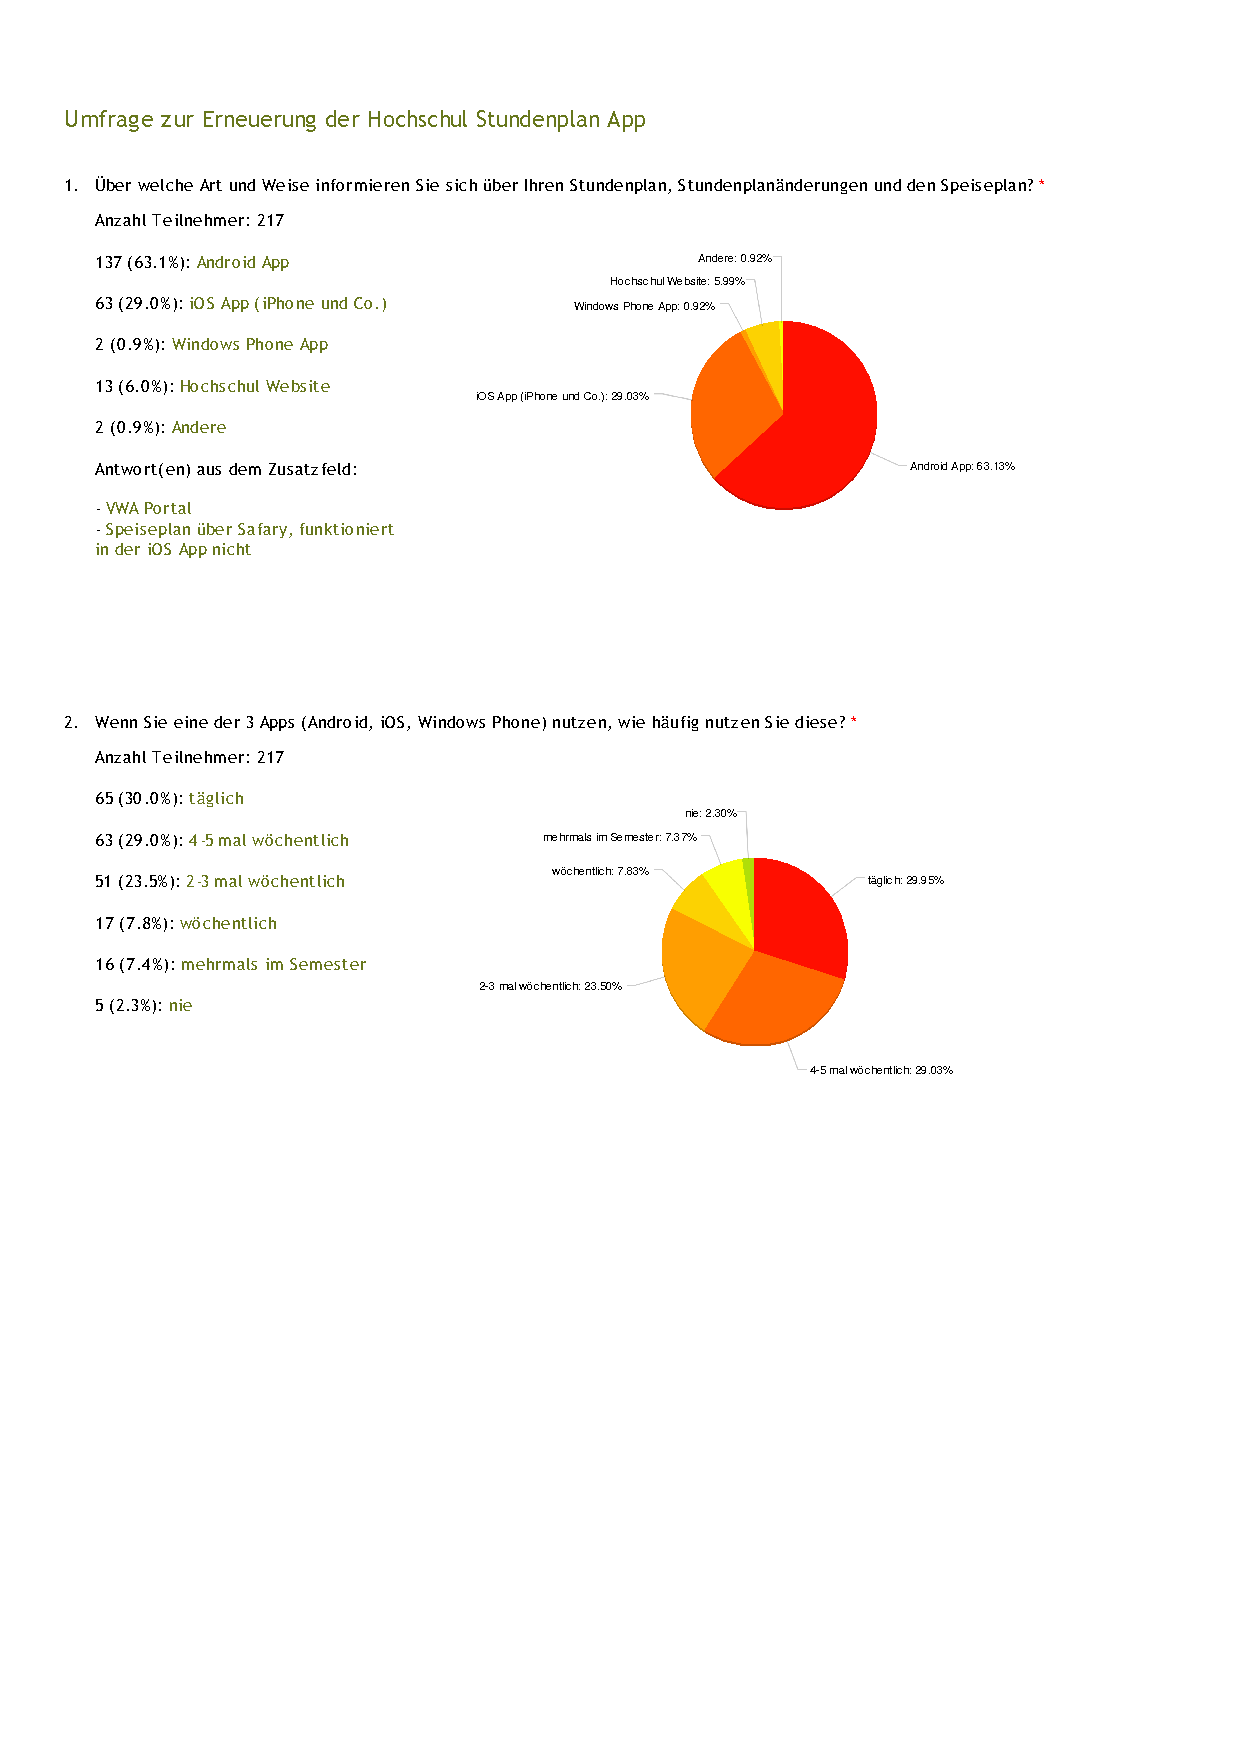
\includegraphics[
    width=\textwidth,
    height=\textheight,
    keepaspectratio
]{Kapiteln/Anhang/Inhalt/DE/umfrage_DE_Page1.pdf}
\vfill
\newpage
\noindent
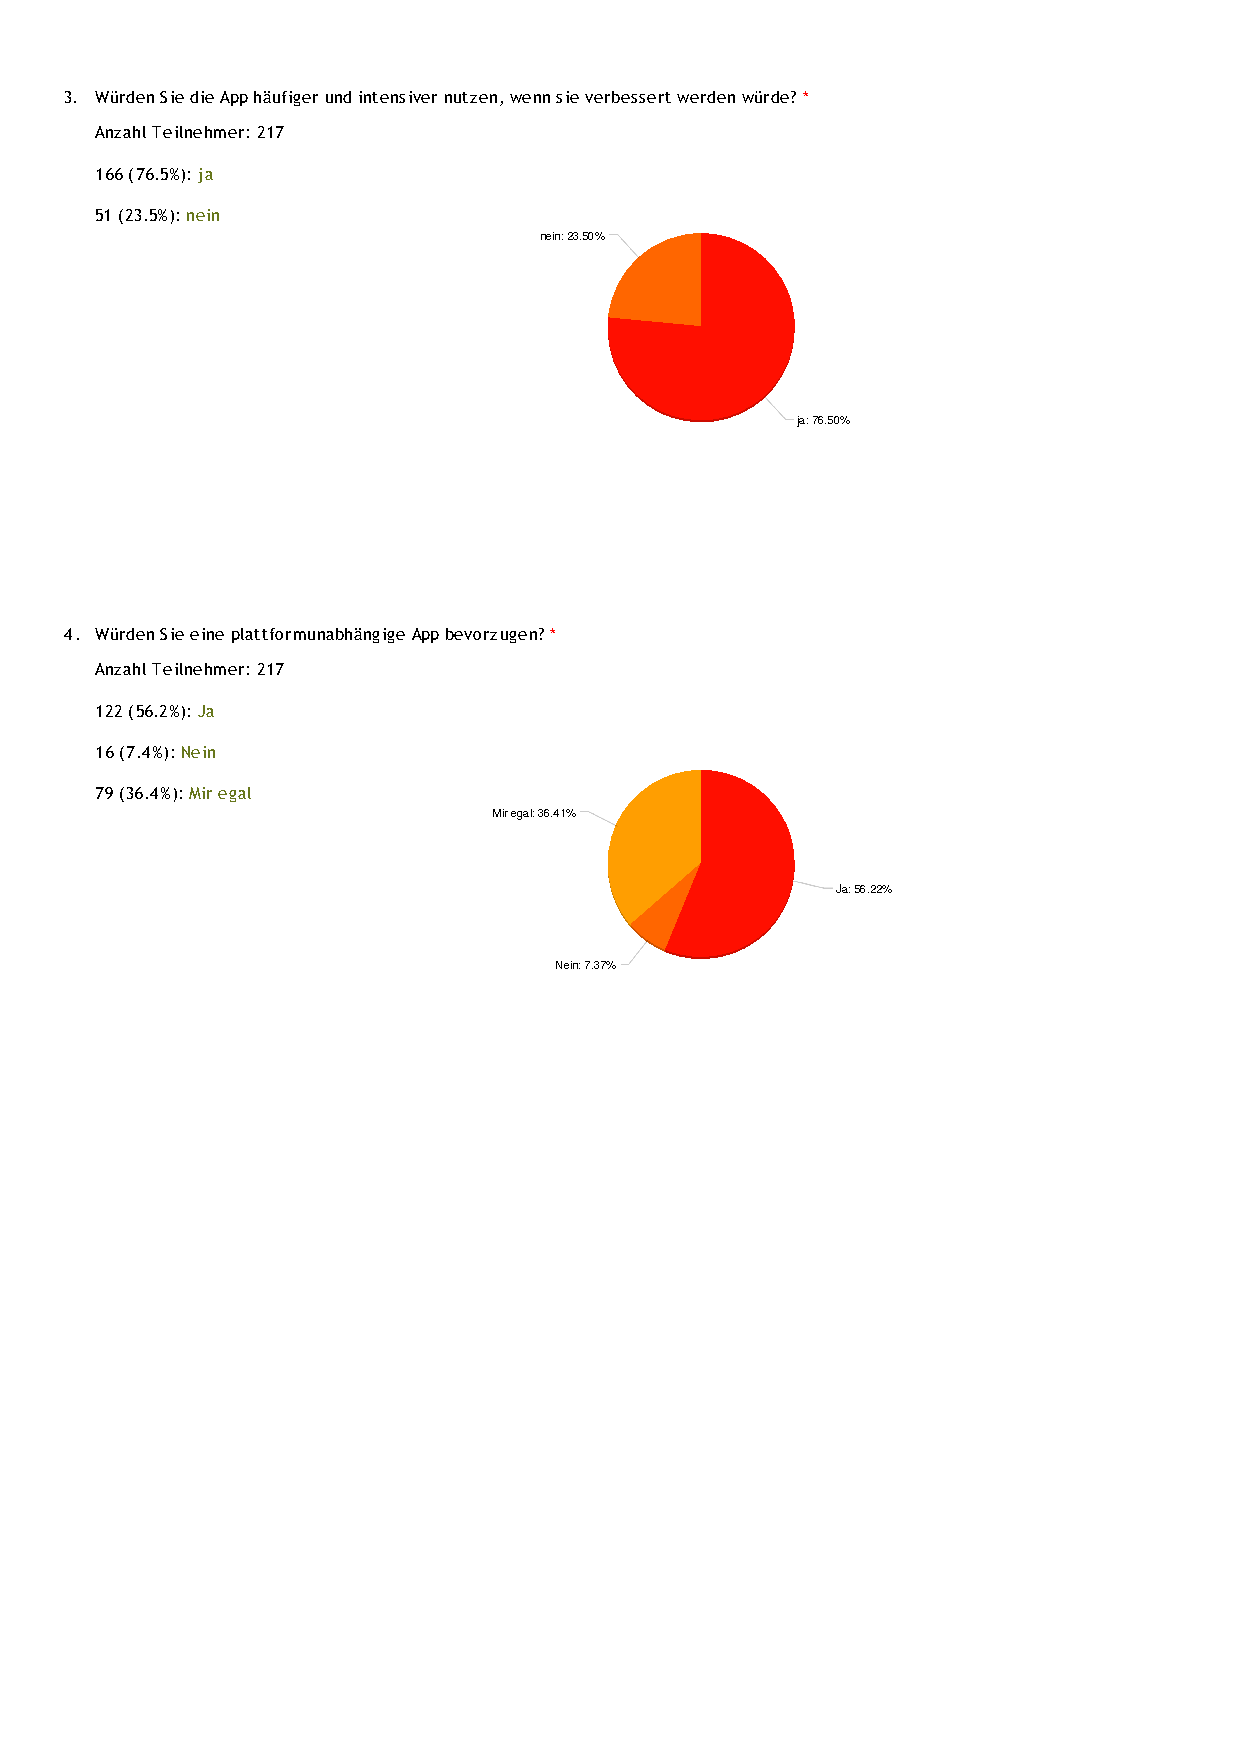
\includegraphics[
    width=\textwidth,
    height=\textheight,
    keepaspectratio
]{Kapiteln/Anhang/Inhalt/DE/umfrage_DE_Page2.pdf}
\vfill
\newpage
\noindent
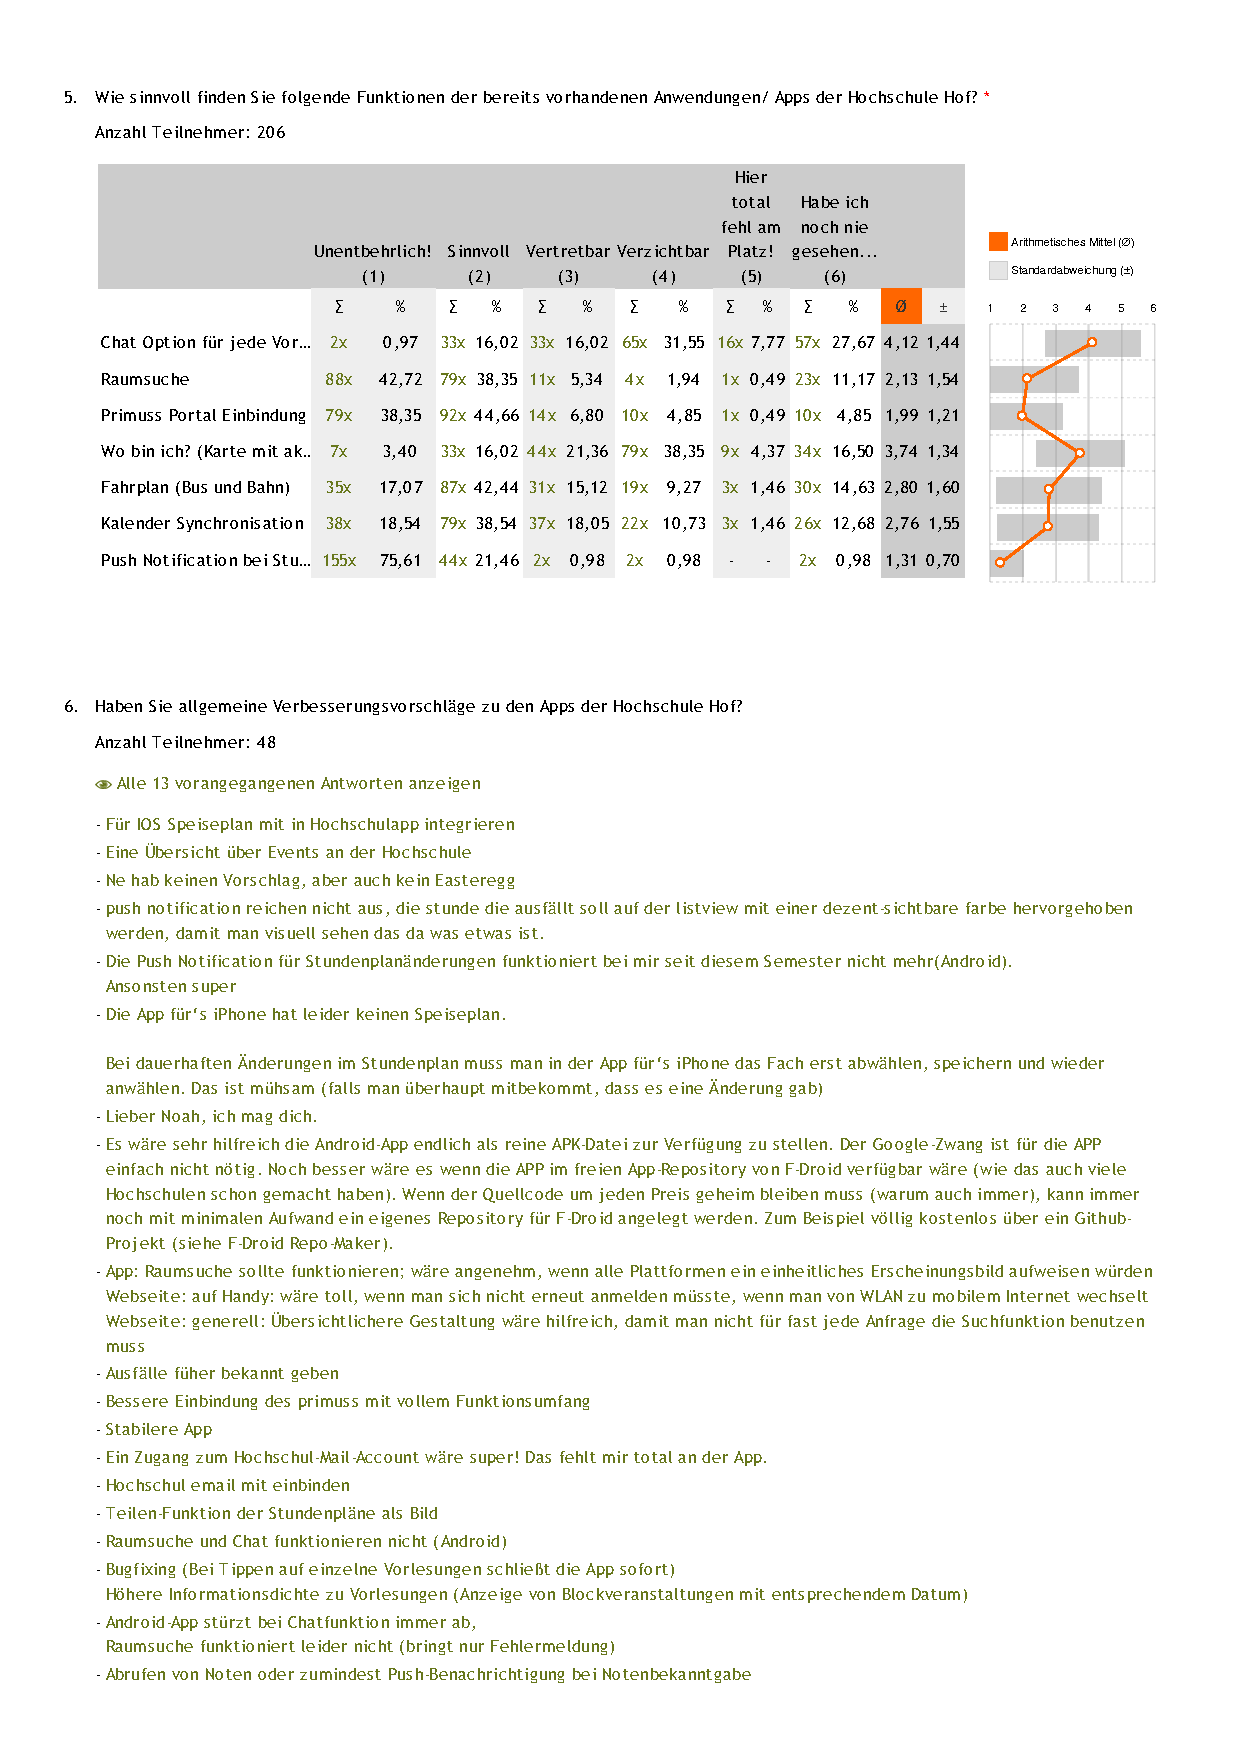
\includegraphics[
    width=\textwidth,
    height=\textheight,
    keepaspectratio
]{Kapiteln/Anhang/Inhalt/DE/umfrage_DE_Page3.pdf}
\vfill
\newpage
\noindent
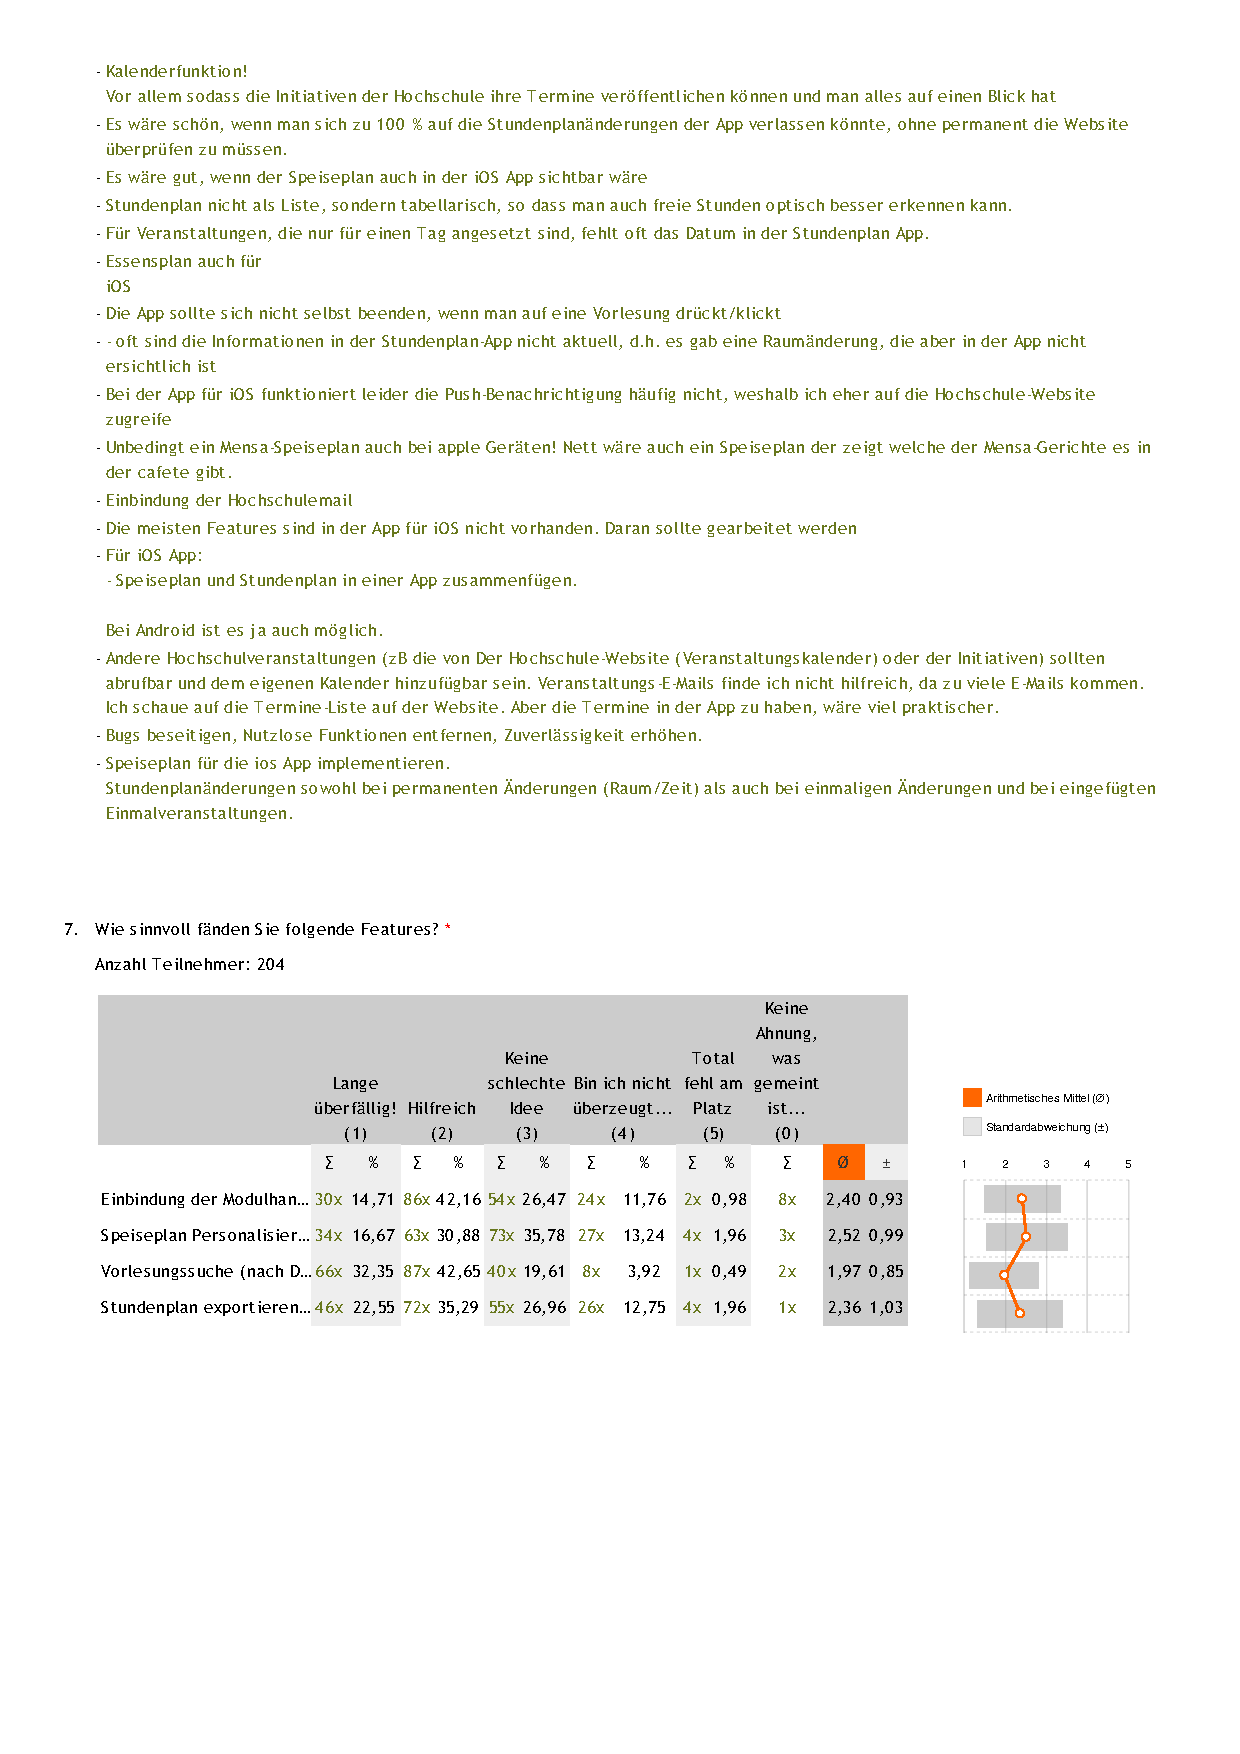
\includegraphics[
    width=\textwidth,
    height=\textheight,
    keepaspectratio
]{Kapiteln/Anhang/Inhalt/DE/umfrage_DE_Page4.pdf}
\vfill
\newpage
\noindent
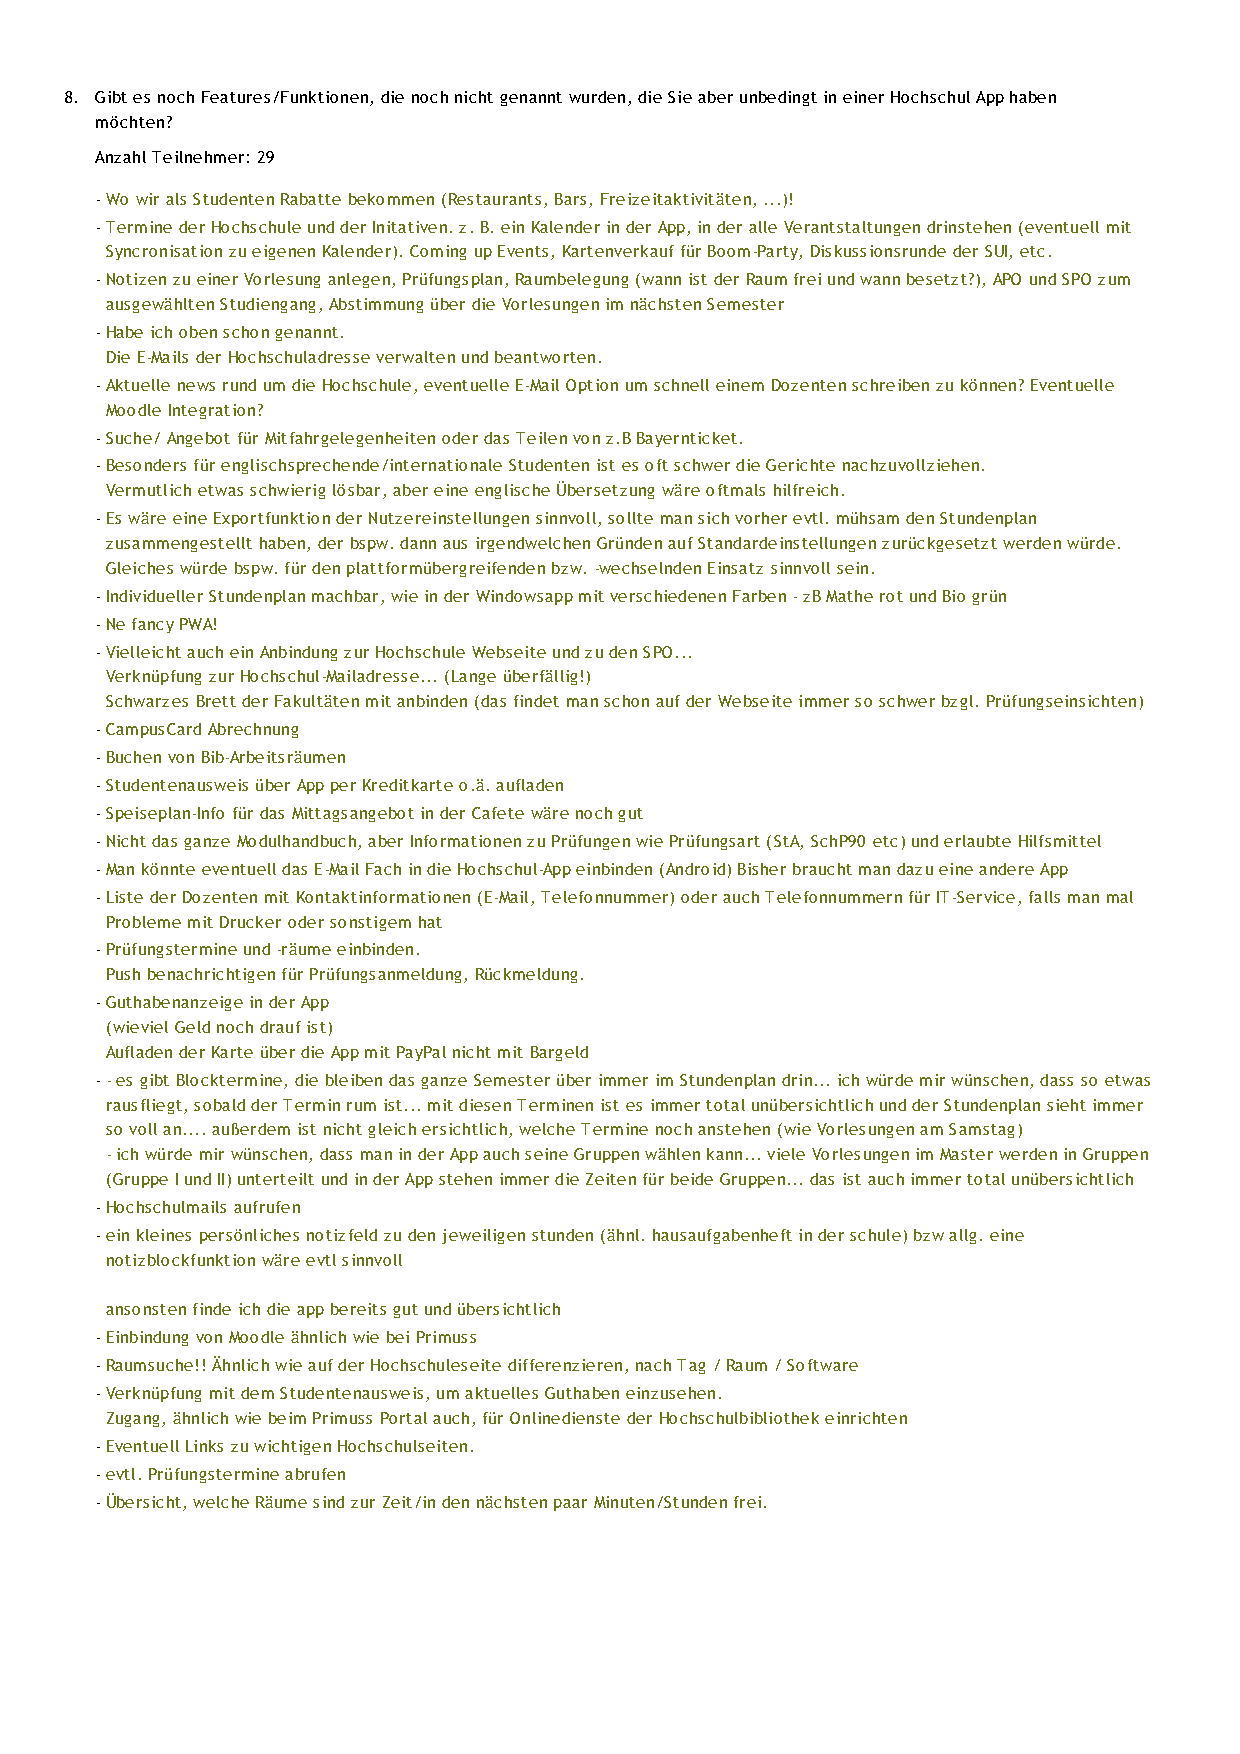
\includegraphics[
    width=\textwidth,
    height=\textheight,
    keepaspectratio
]{Kapiteln/Anhang/Inhalt/DE/umfrage_DE_Page5.pdf}
\vfill
\newpage
\noindent
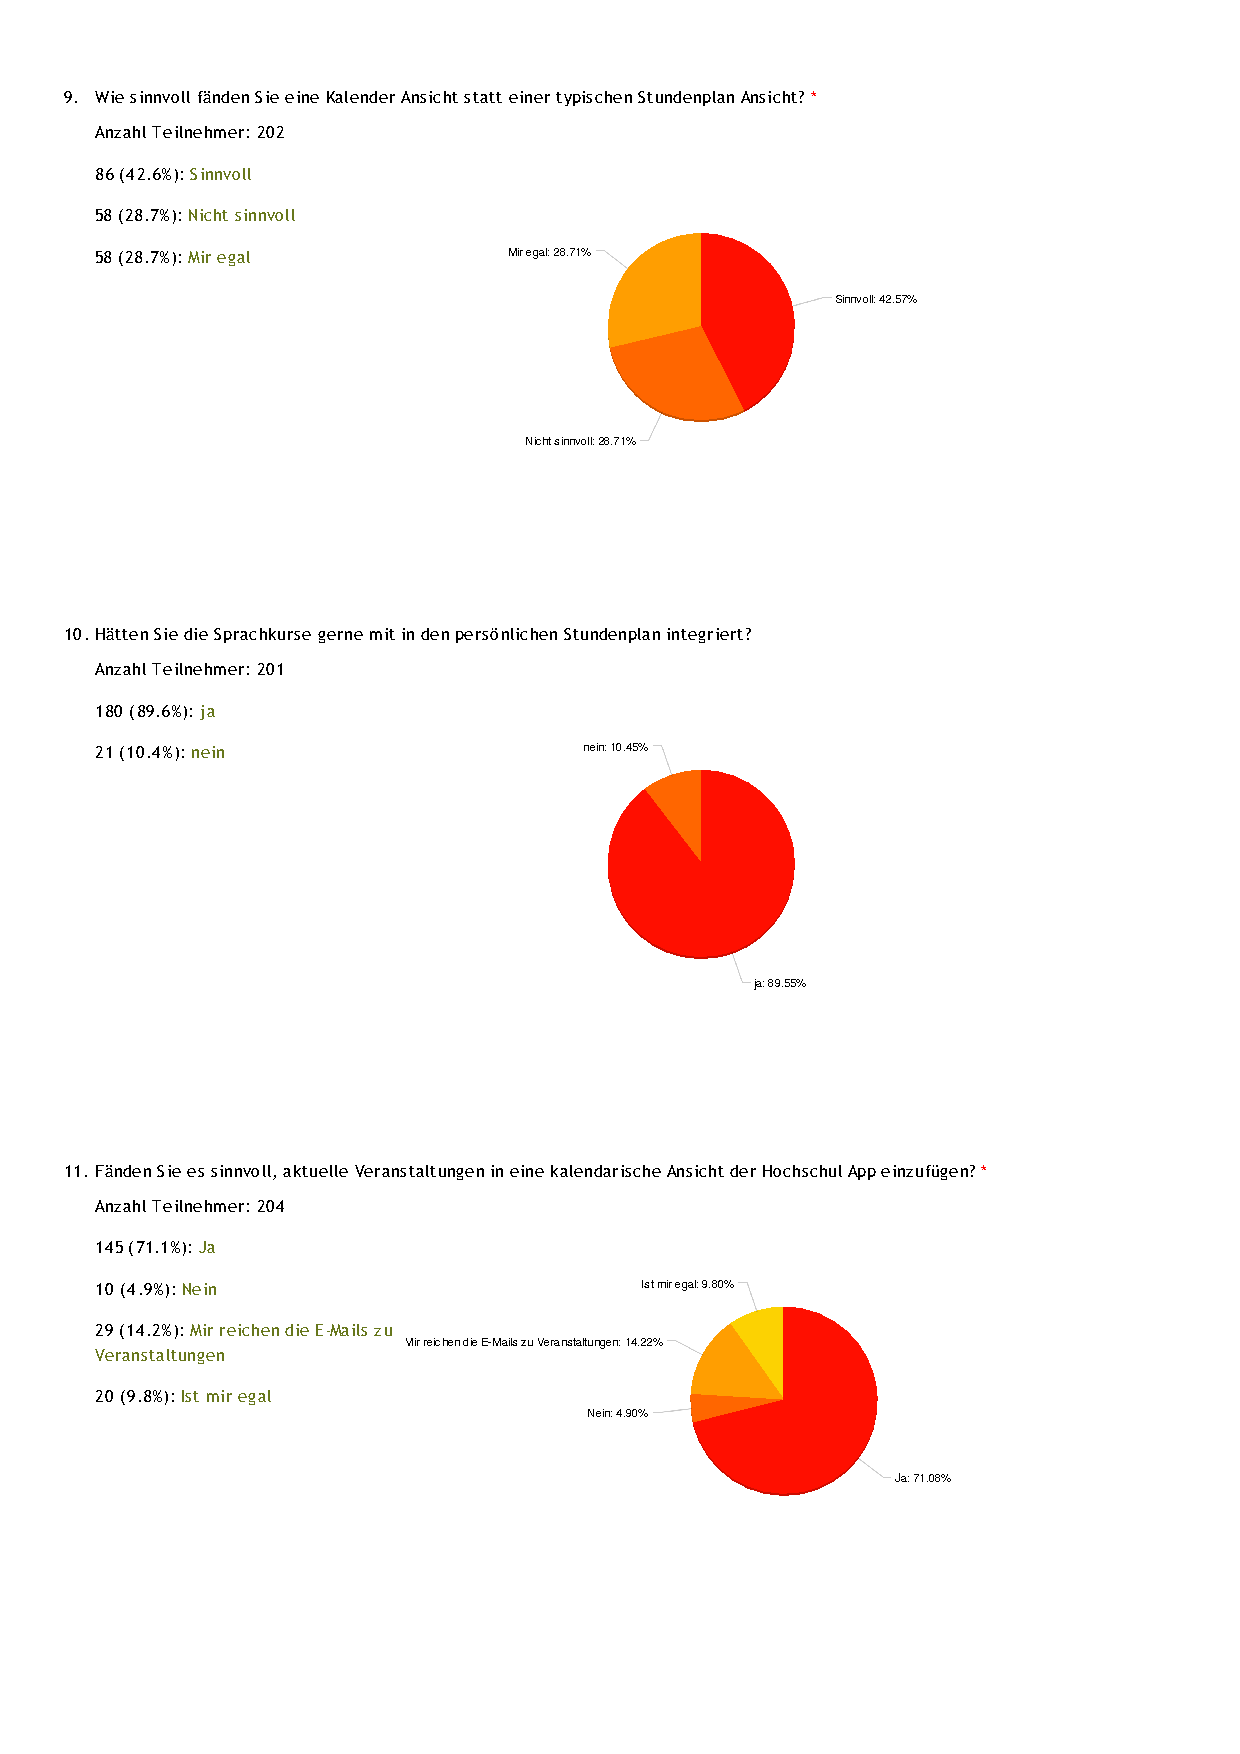
\includegraphics[
    width=\textwidth,
    height=\textheight,
    keepaspectratio
]{Kapiteln/Anhang/Inhalt/DE/umfrage_DE_Page6.pdf}
\vfill
\newpage
\noindent
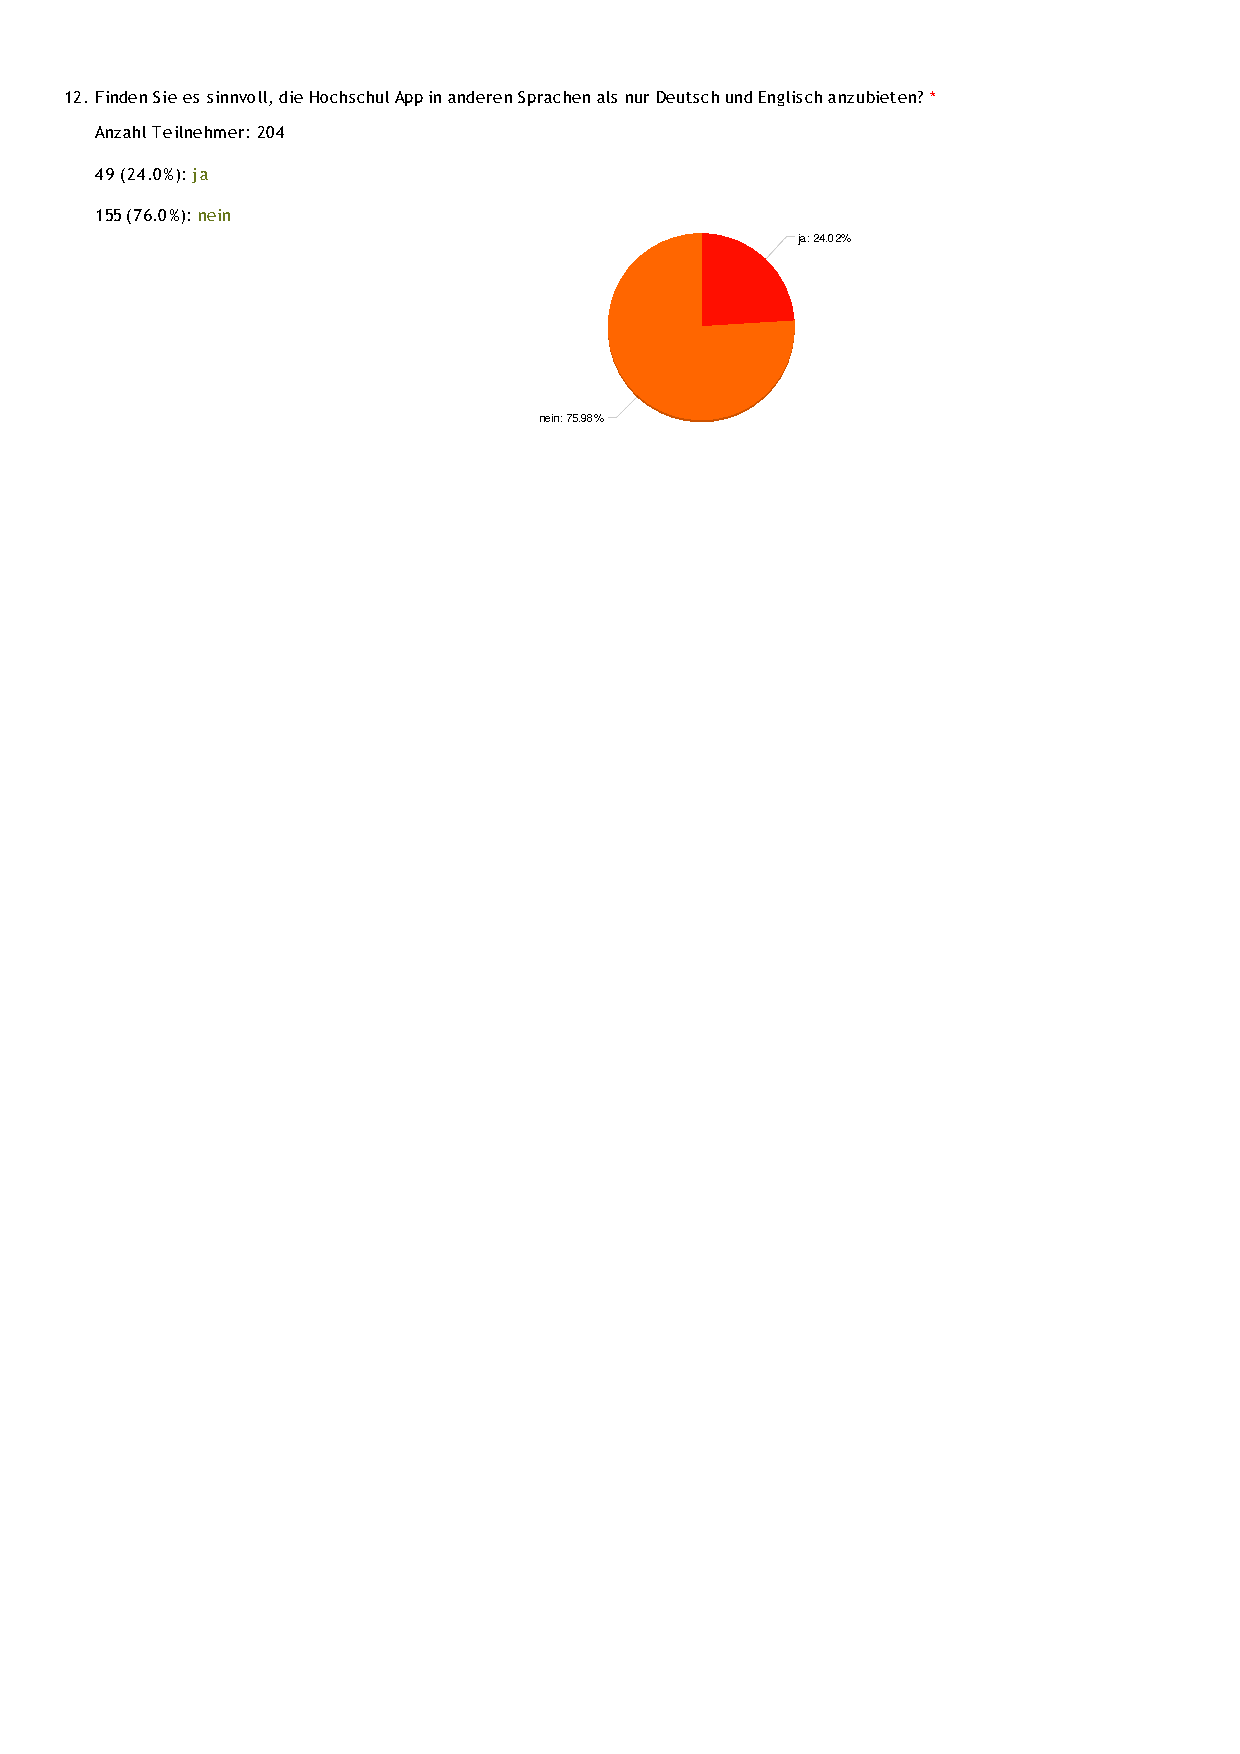
\includegraphics[
    width=\textwidth,
    height=\textheight,
    keepaspectratio
]{Kapiteln/Anhang/Inhalt/DE/umfrage_DE_Page7.pdf}
\vfill
\newpage
\noindent
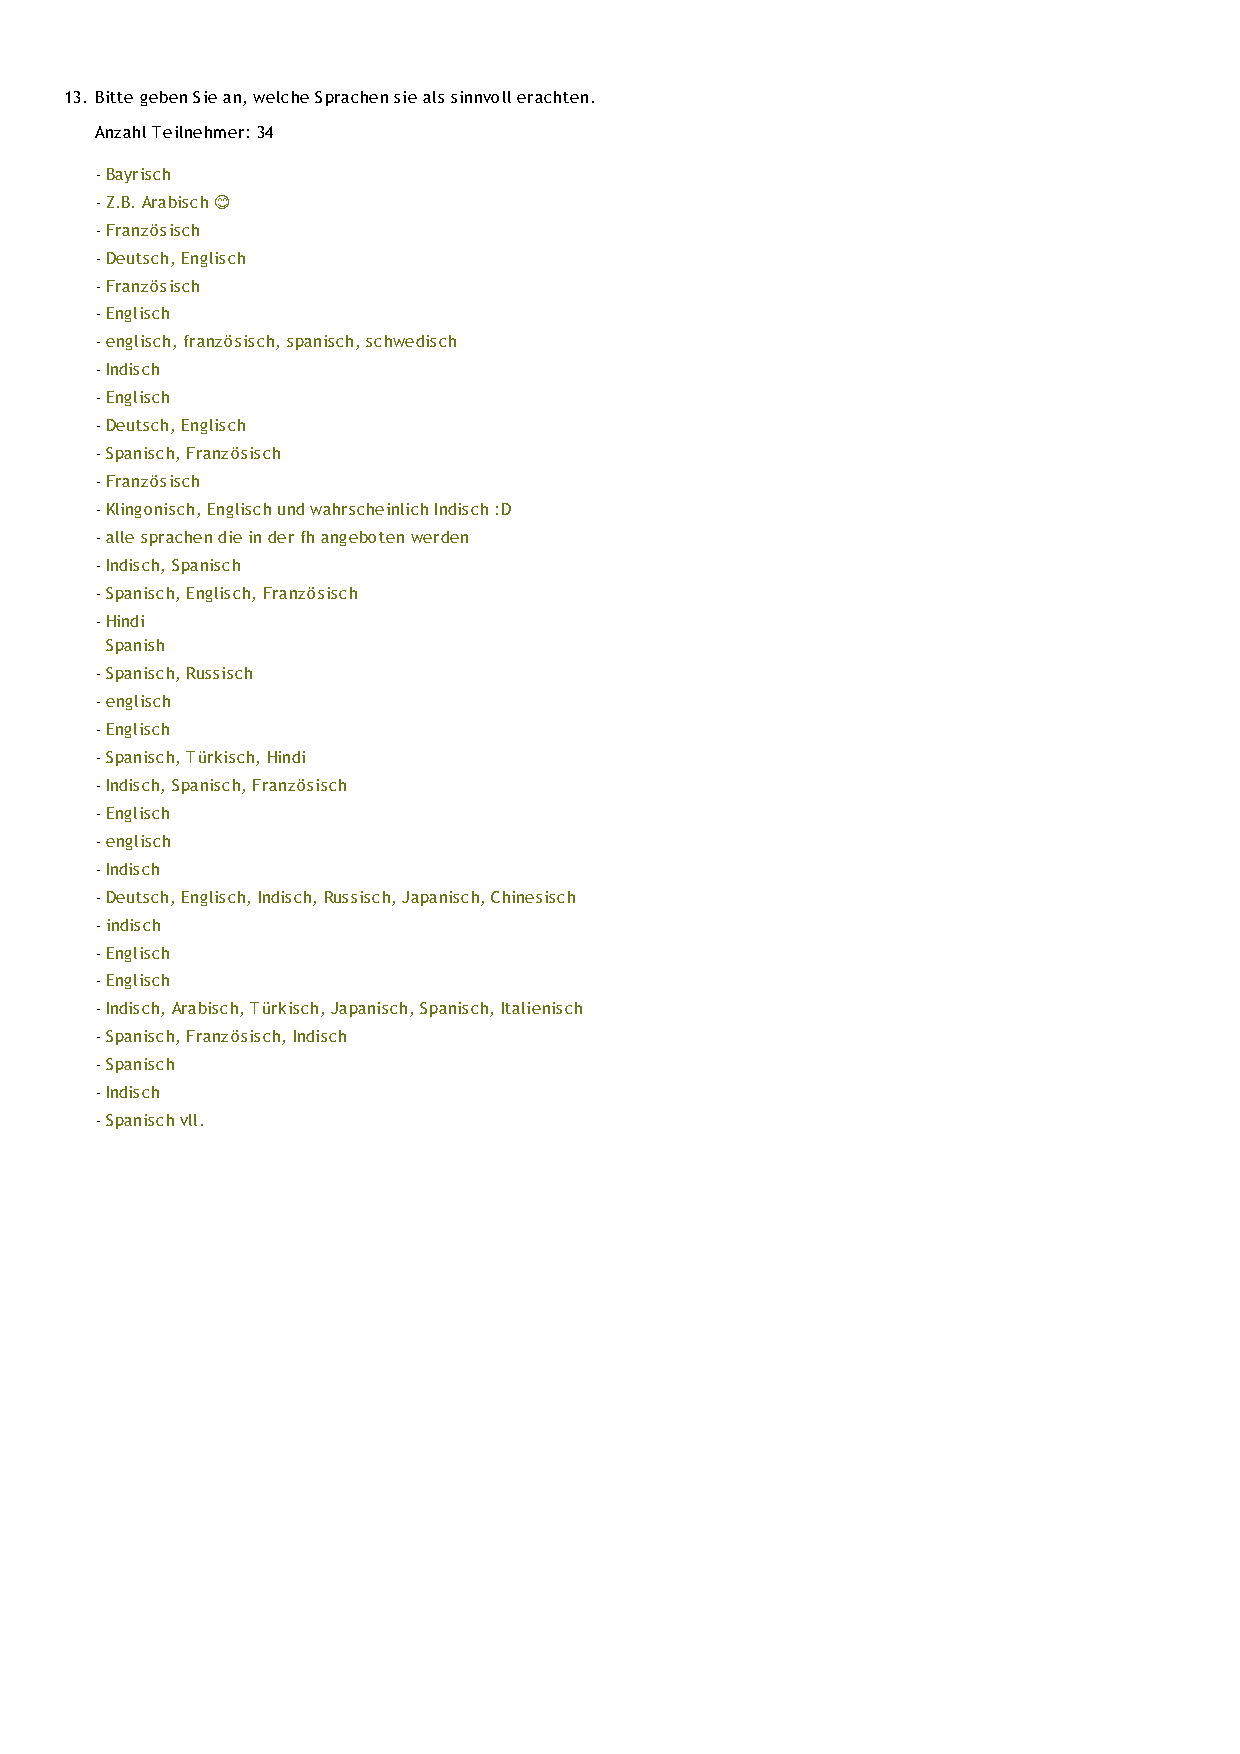
\includegraphics[
    width=\textwidth,
    height=\textheight,
    keepaspectratio
]{Kapiteln/Anhang/Inhalt/DE/umfrage_DE_Page8.pdf}
\vfill
\newpage
\noindent
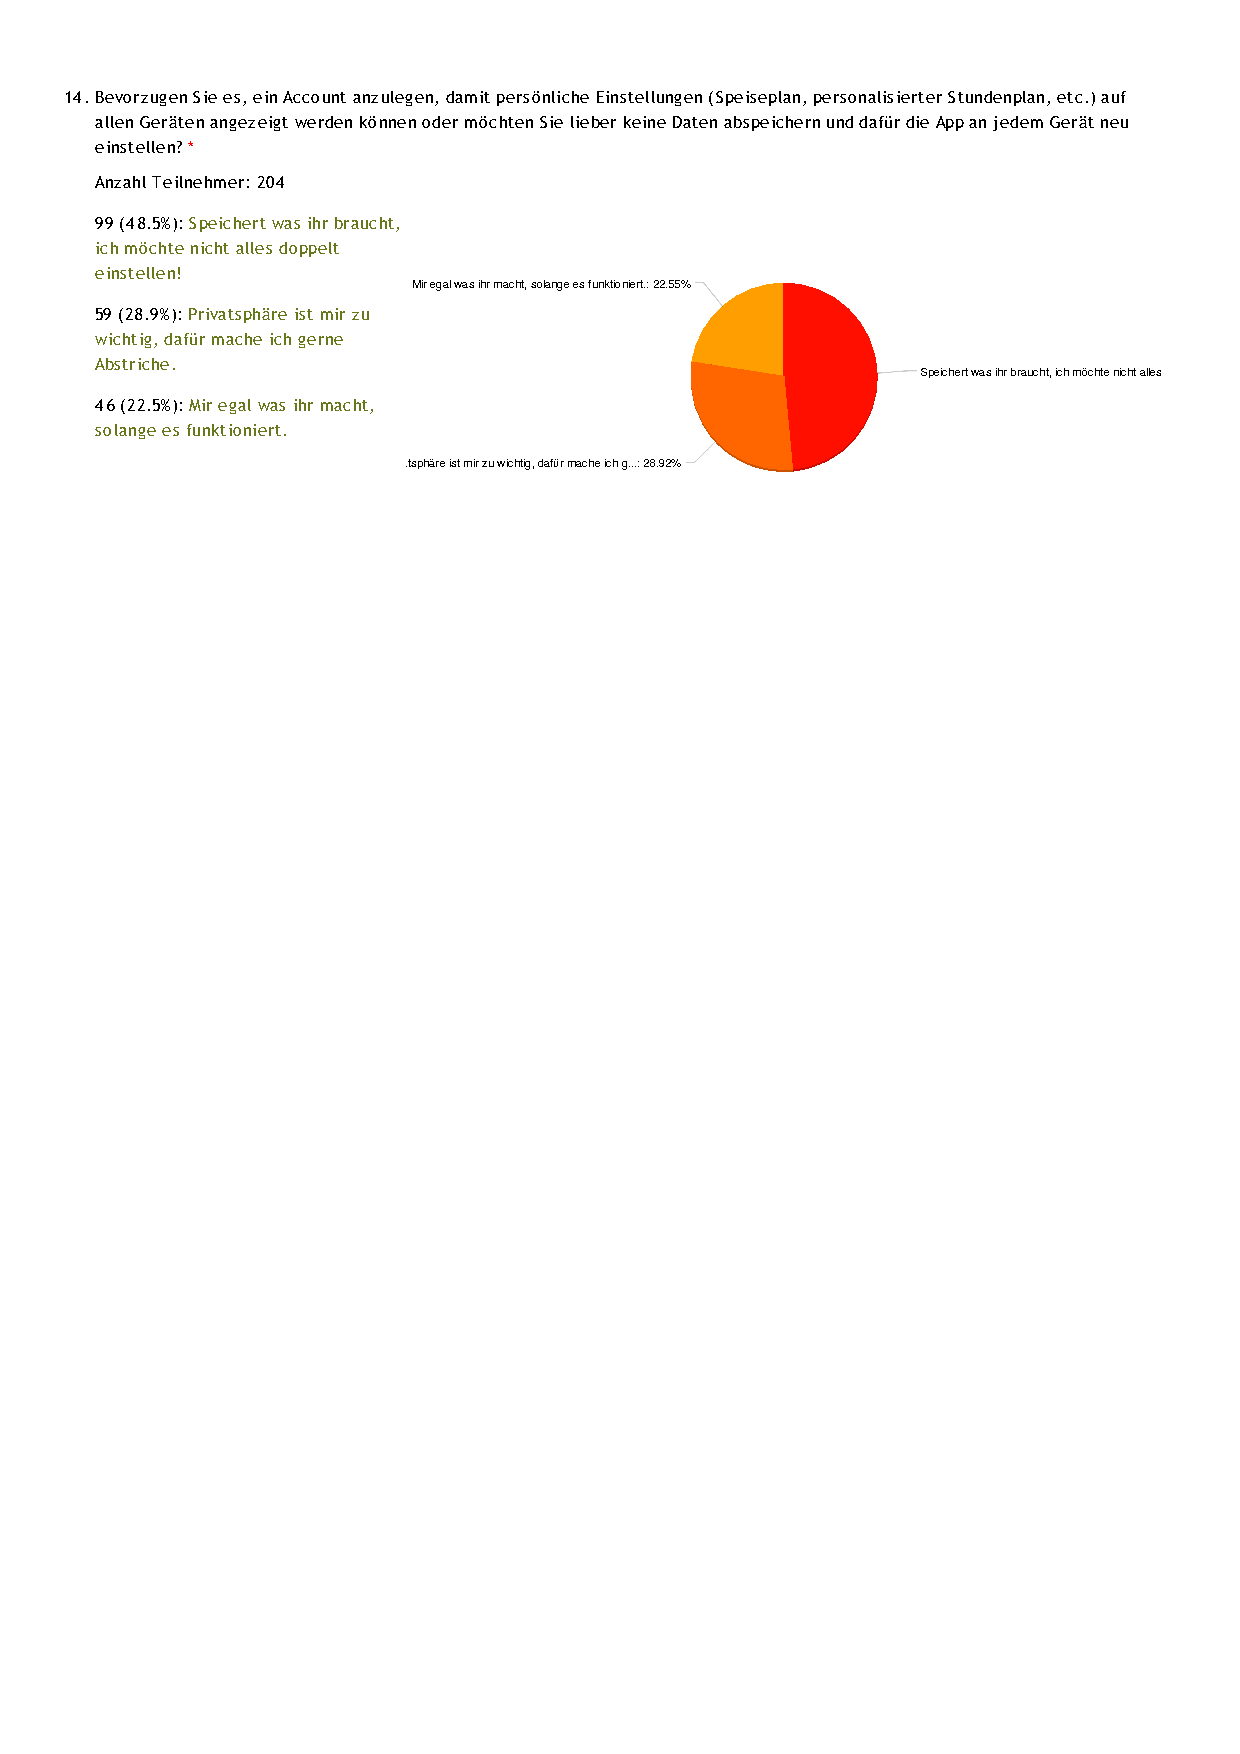
\includegraphics[
    width=\textwidth,
    height=\textheight,
    keepaspectratio
]{Kapiteln/Anhang/Inhalt/DE/umfrage_DE_Page9.pdf}
\vfill
\newpage
\noindent
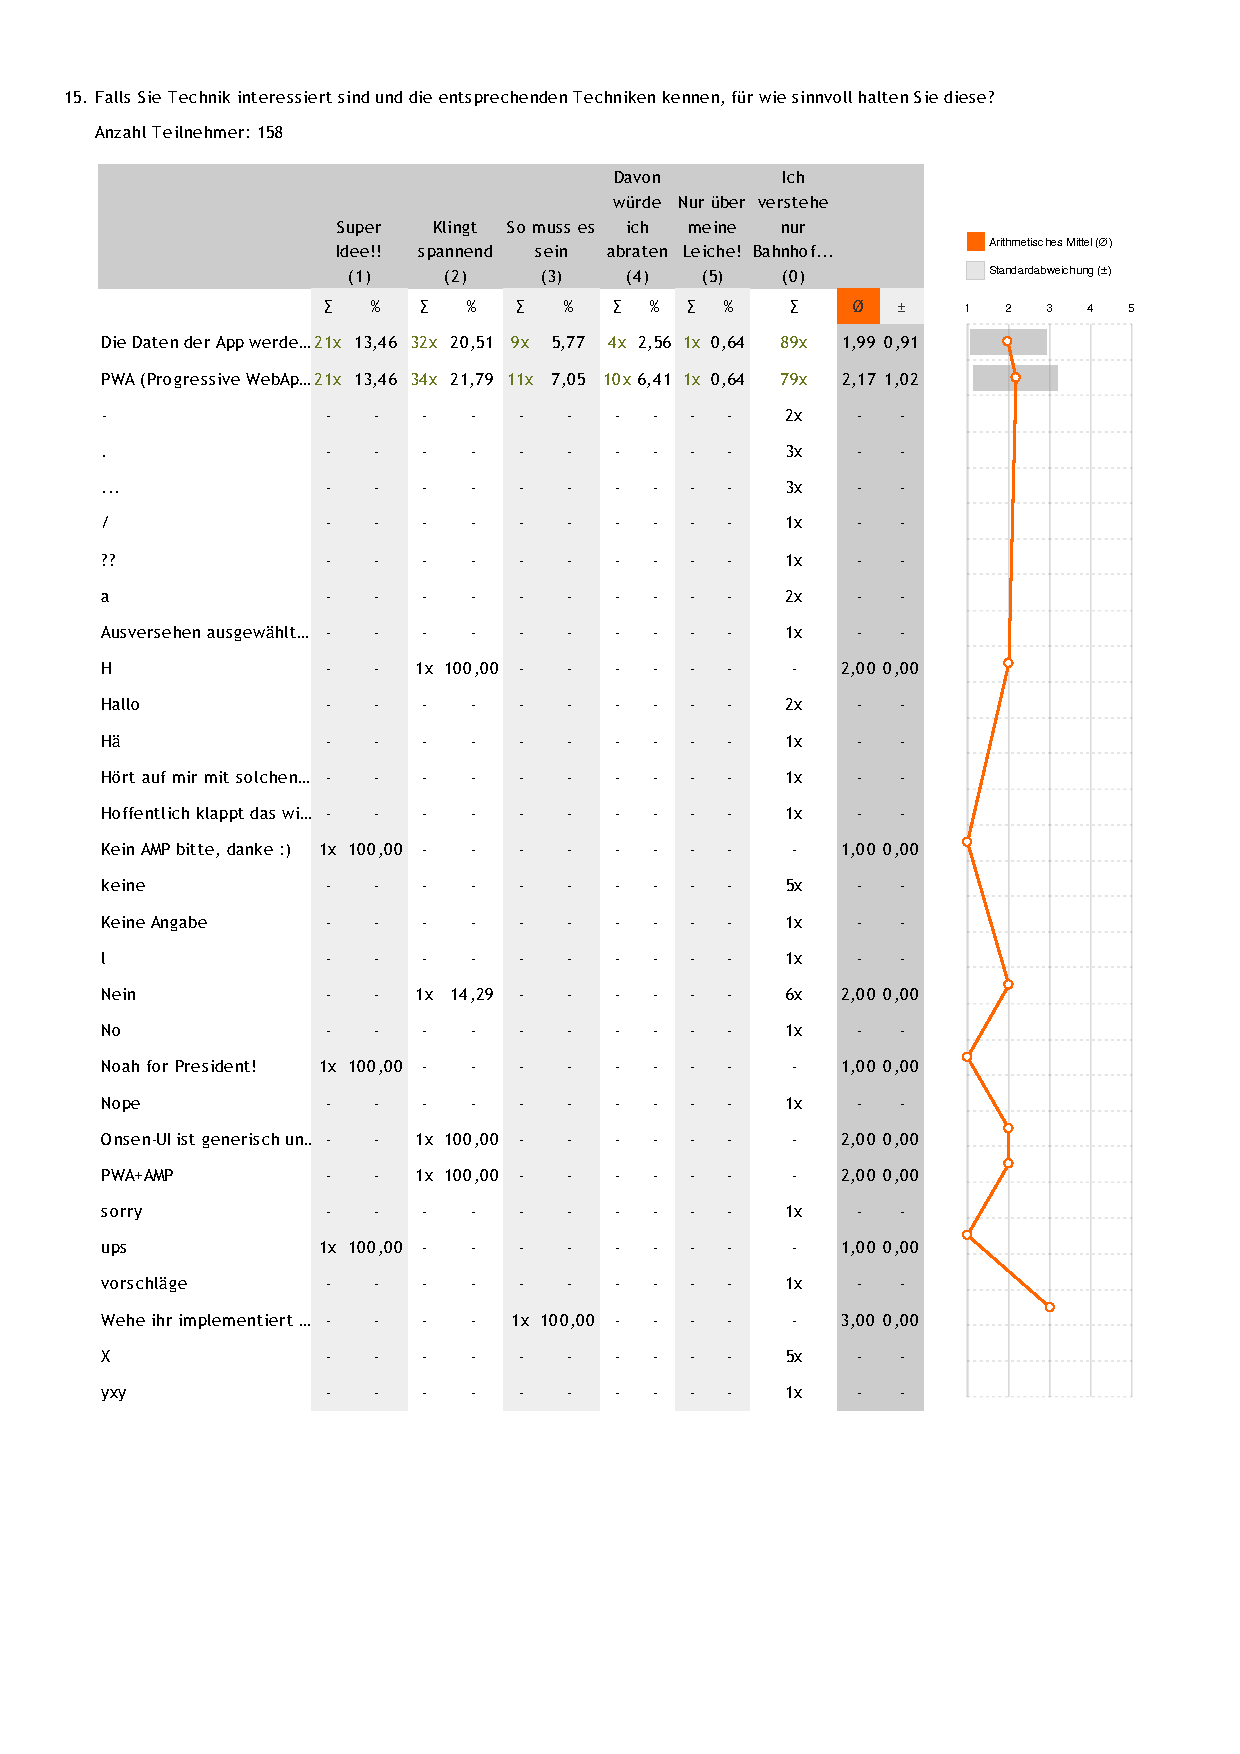
\includegraphics[
    width=\textwidth,
    height=\textheight,
    keepaspectratio
]{Kapiteln/Anhang/Inhalt/DE/umfrage_DE_Page10.pdf}
\vfill
\newpage

\section*{Internationale Umfrage}
\addcontentsline{toc}{subsection}{Internationale Umfrage}

\noindent
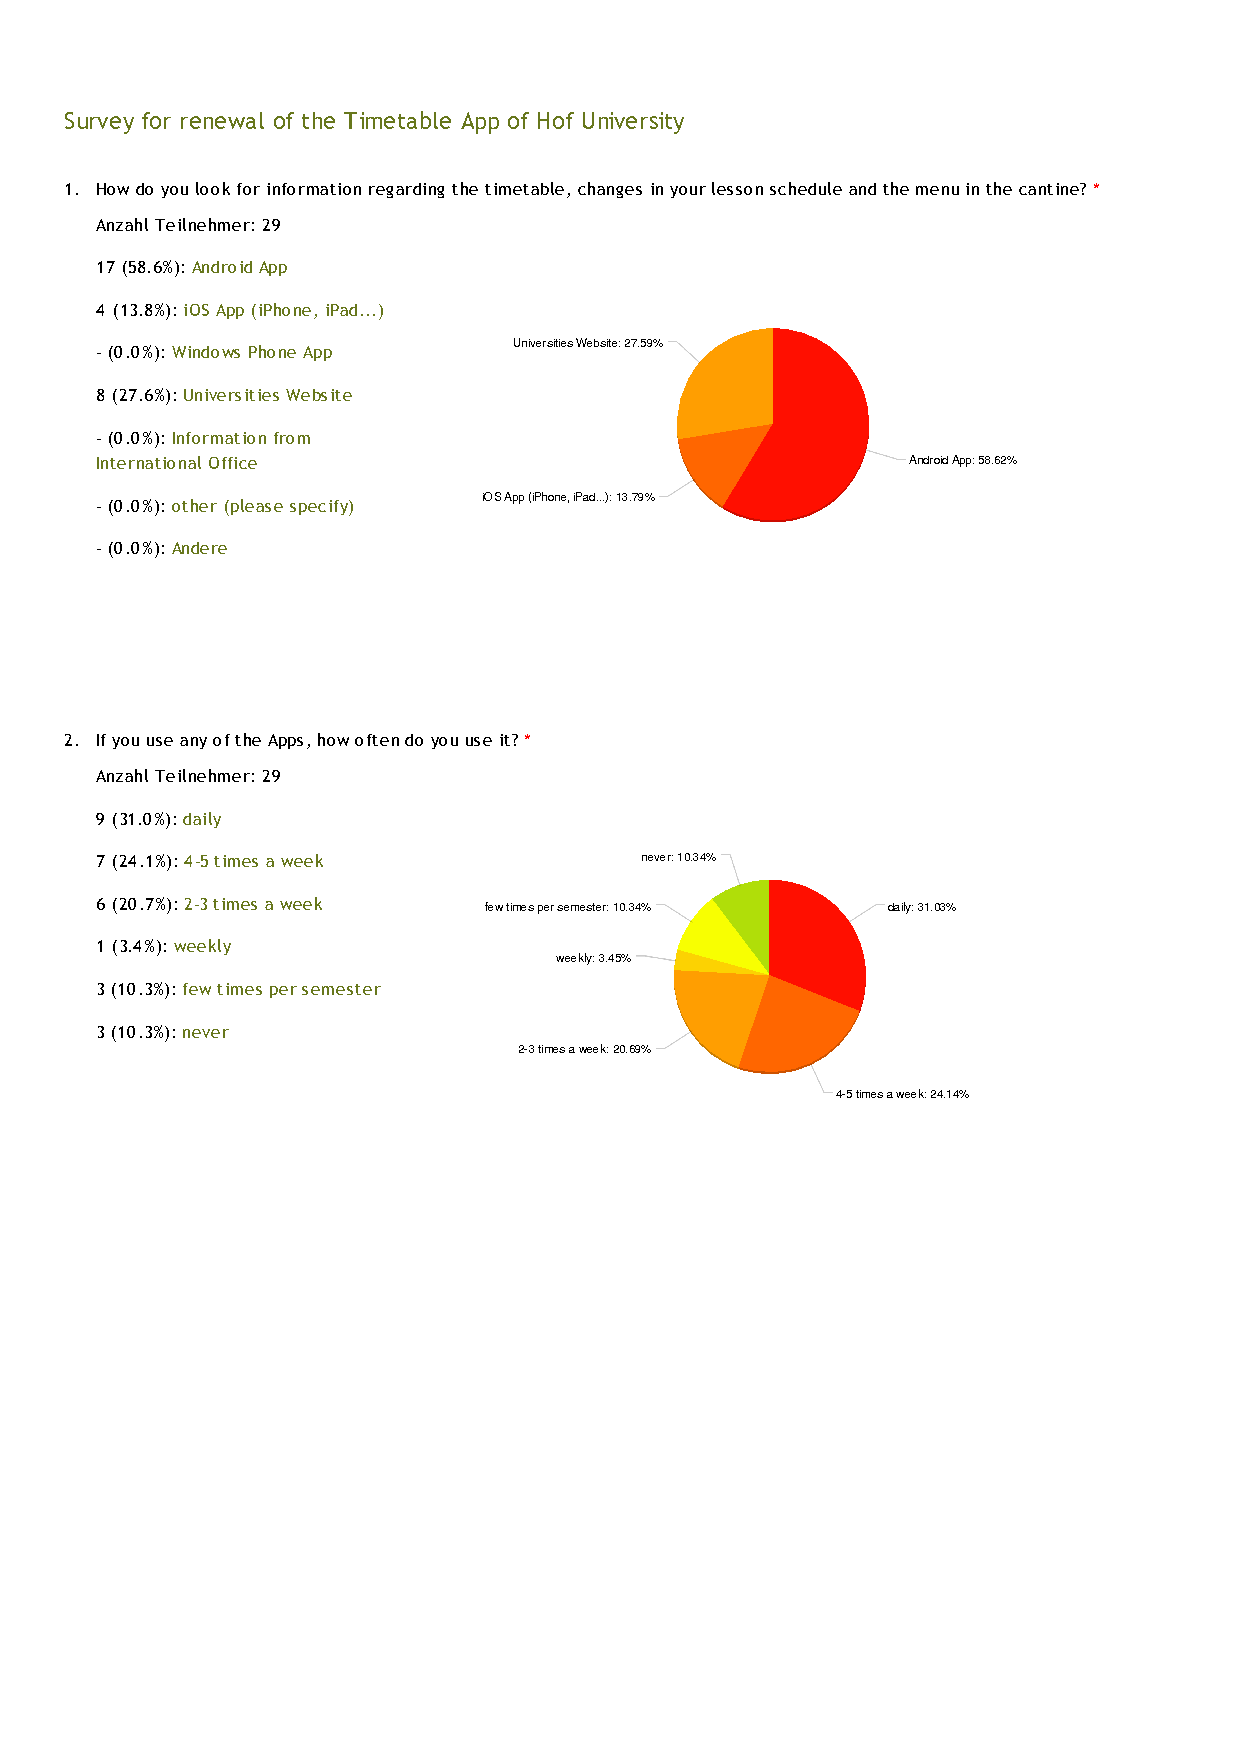
\includegraphics[
    width=\textwidth,
    height=\textheight,
    keepaspectratio
]{Kapiteln/Anhang/Inhalt/EN/survey_EN_Page1.pdf}
\vfill
\newpage
\noindent
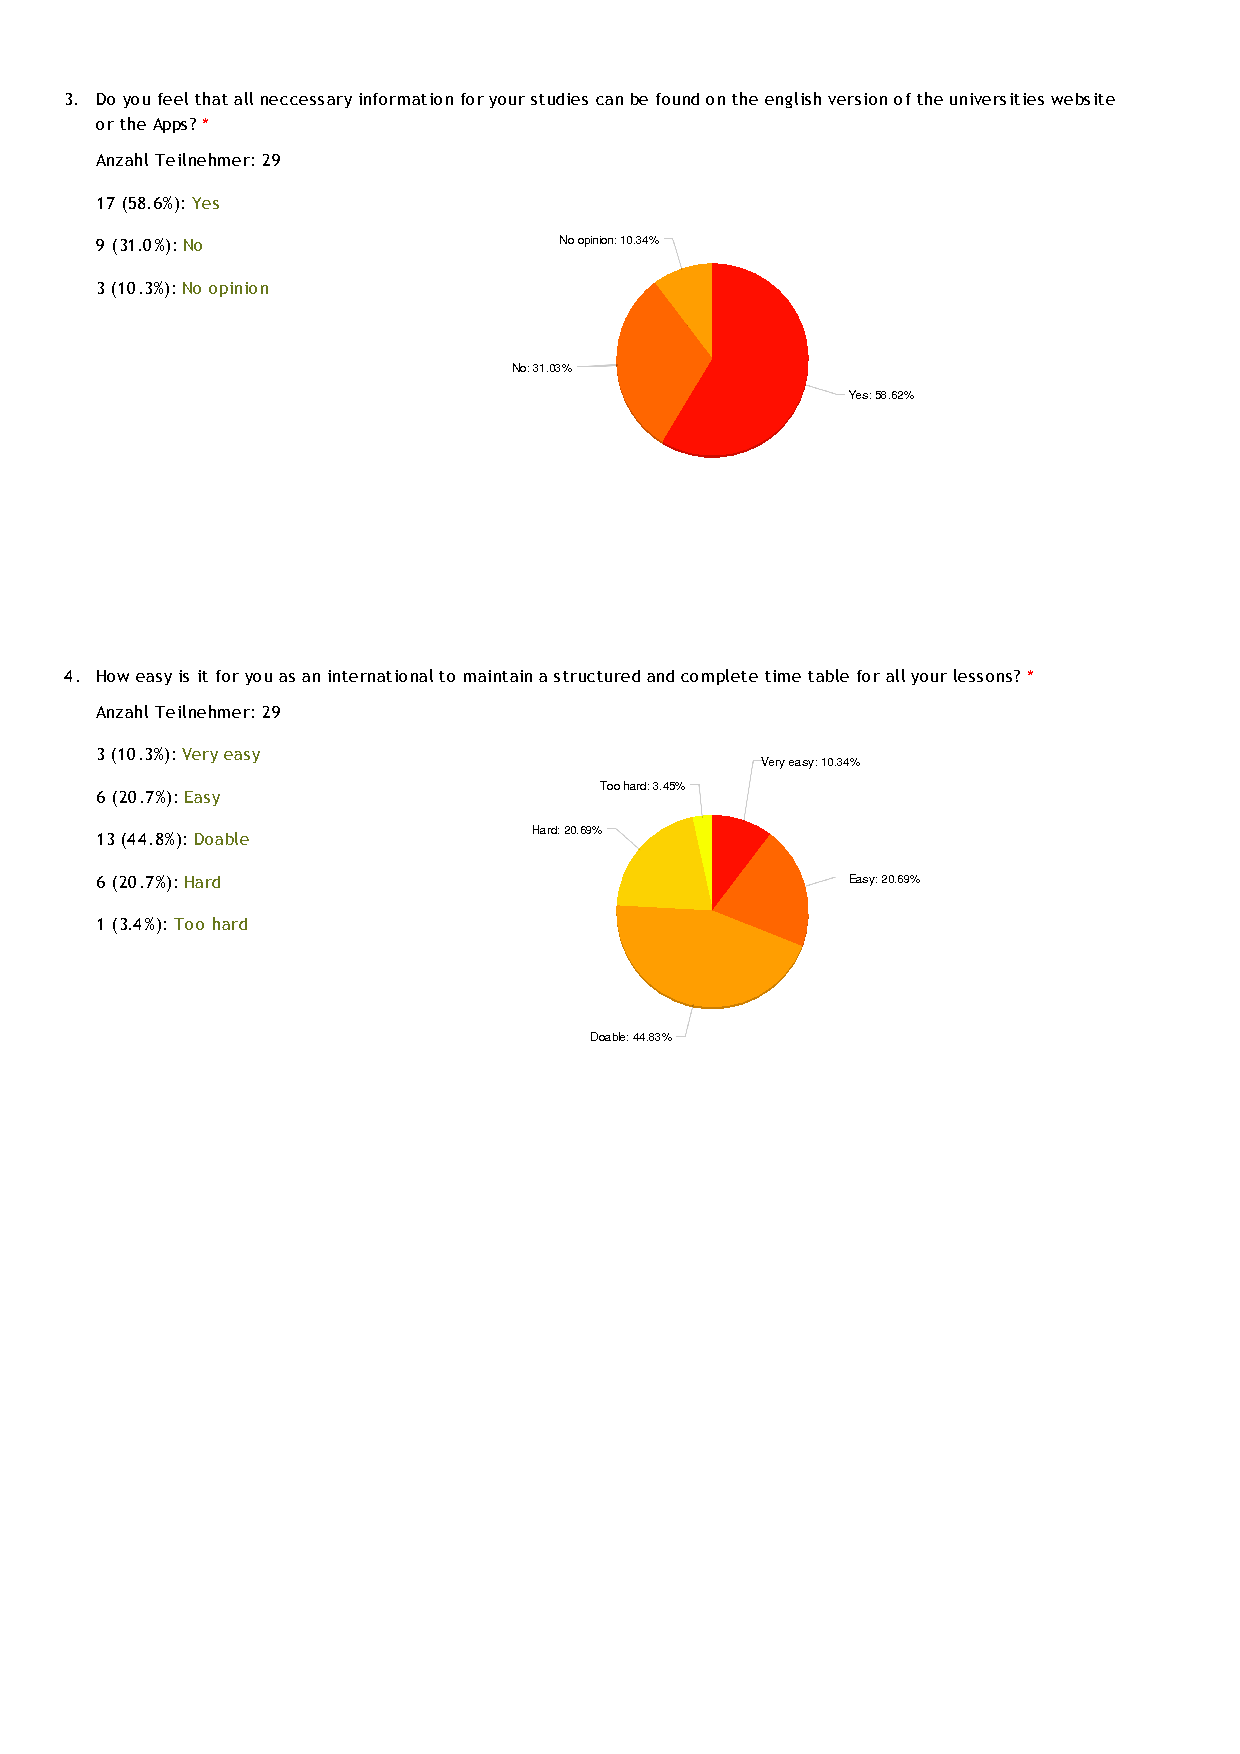
\includegraphics[
    width=\textwidth,
    height=\textheight,
    keepaspectratio
]{Kapiteln/Anhang/Inhalt/EN/survey_EN_Page2.pdf}
\vfill
\newpage
\noindent
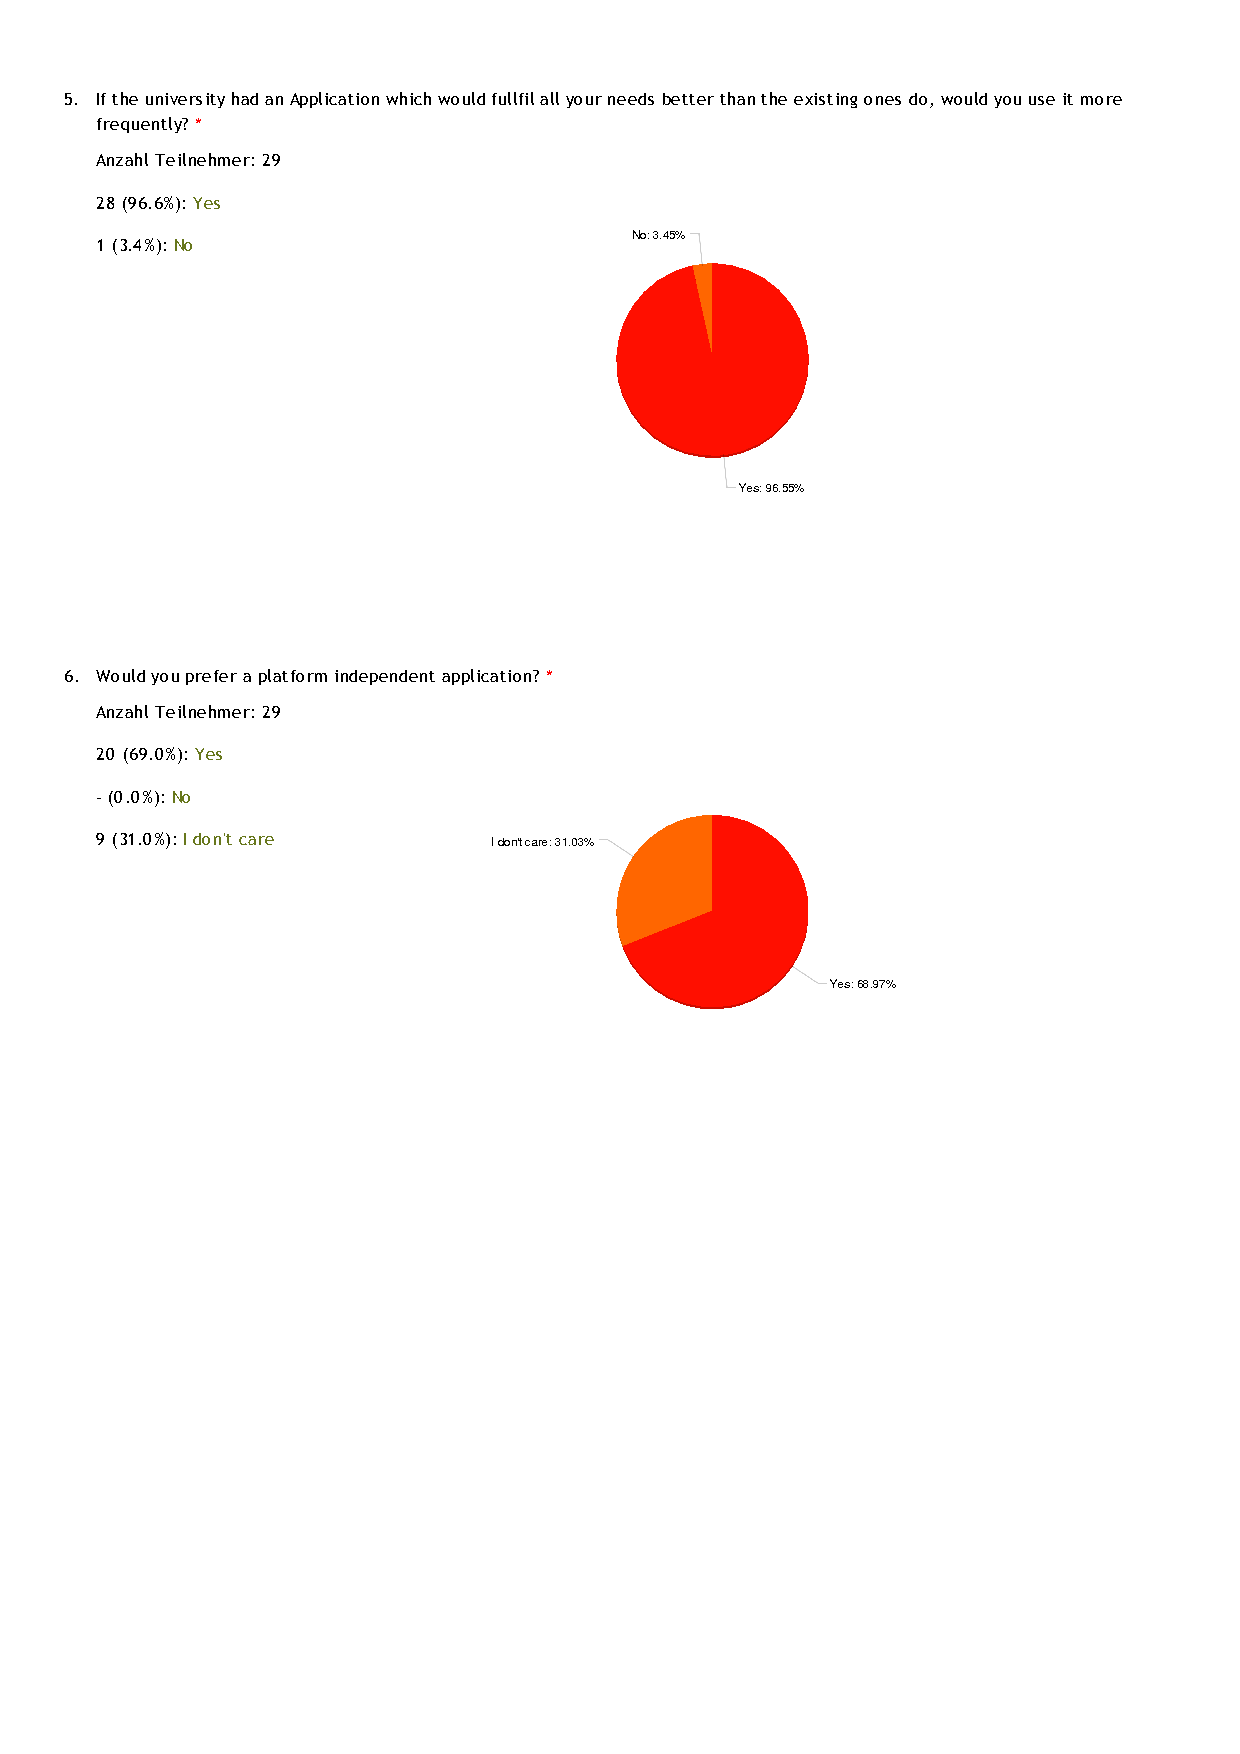
\includegraphics[
    width=\textwidth,
    height=\textheight,
    keepaspectratio
]{Kapiteln/Anhang/Inhalt/EN/survey_EN_Page3.pdf}
\vfill
\newpage
\noindent
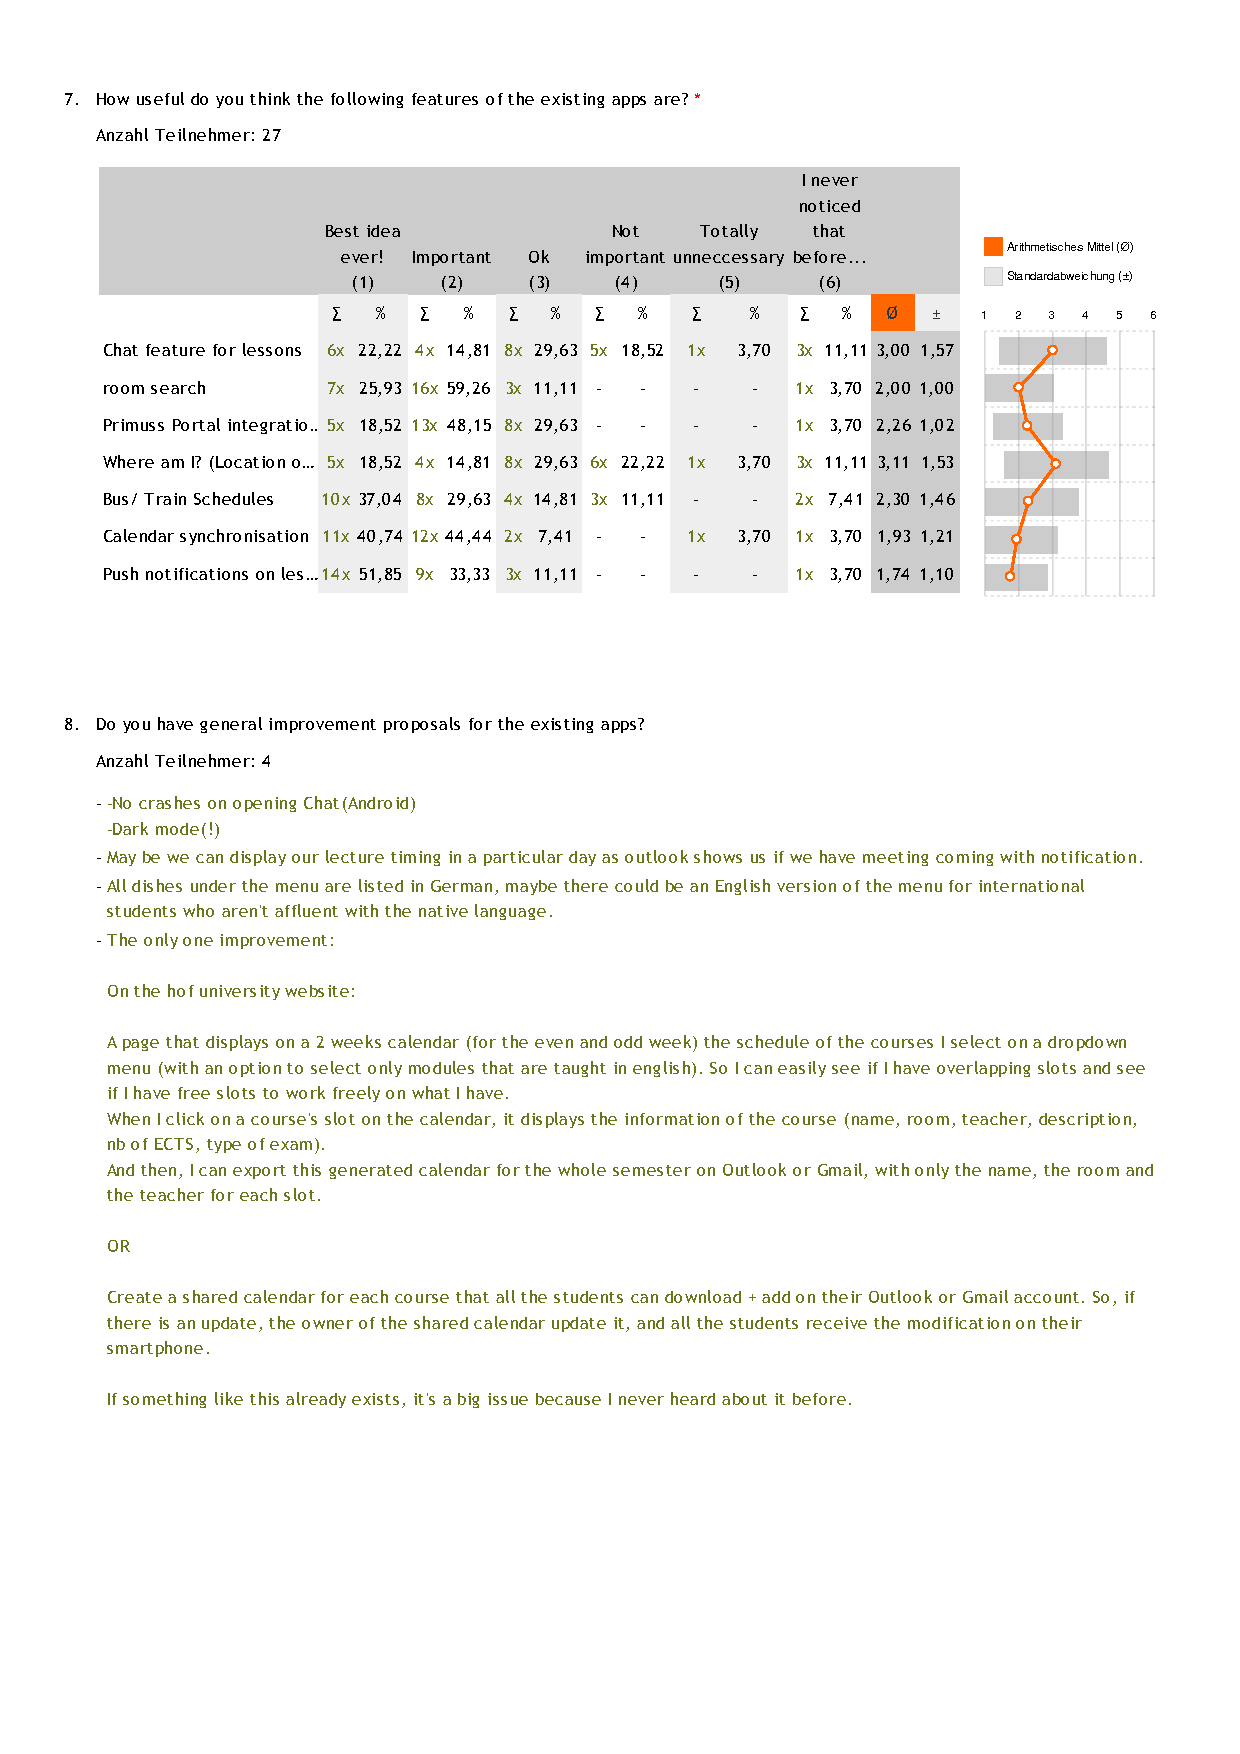
\includegraphics[
    width=\textwidth,
    height=\textheight,
    keepaspectratio
]{Kapiteln/Anhang/Inhalt/EN/survey_EN_Page4.pdf}
\vfill
\newpage
\noindent
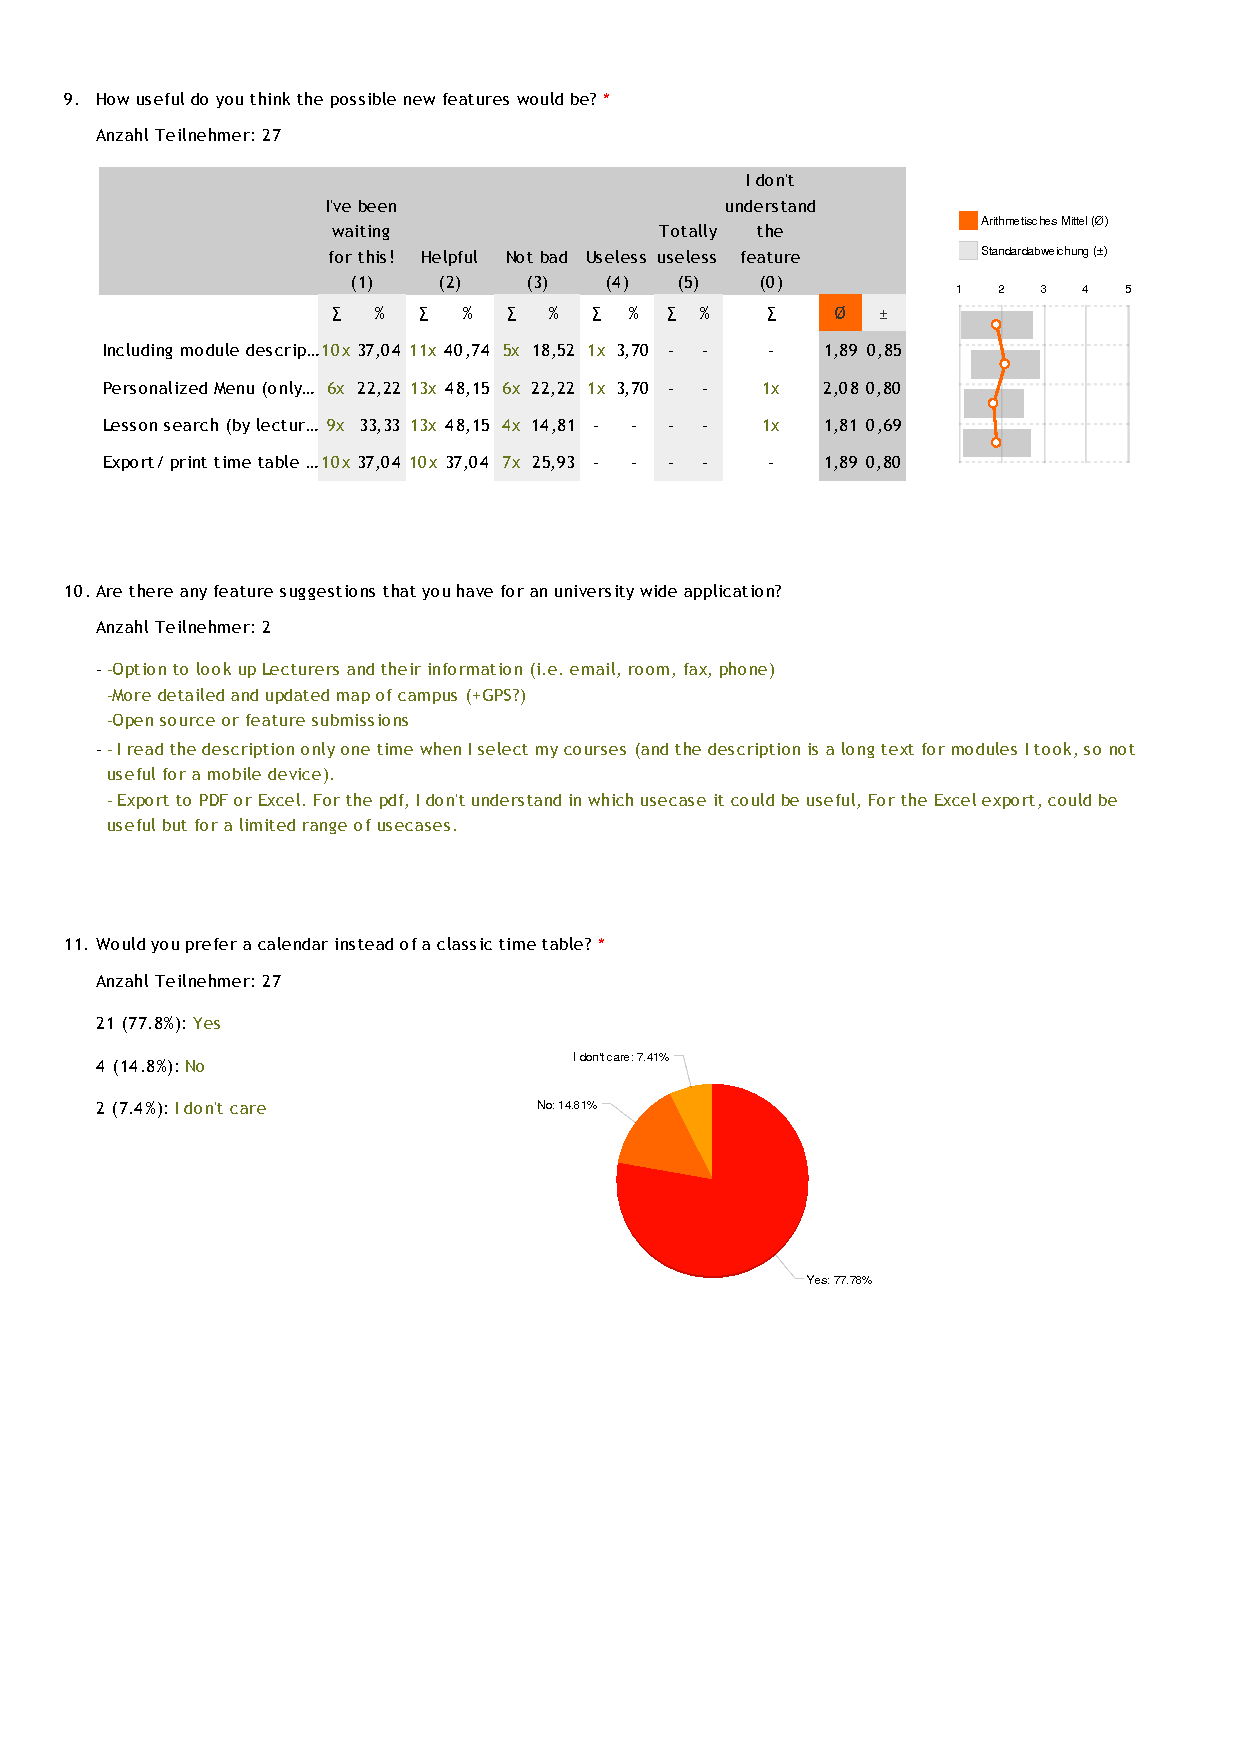
\includegraphics[
    width=\textwidth,
    height=\textheight,
    keepaspectratio
]{Kapiteln/Anhang/Inhalt/EN/survey_EN_Page5.pdf}
\vfill
\newpage
\noindent
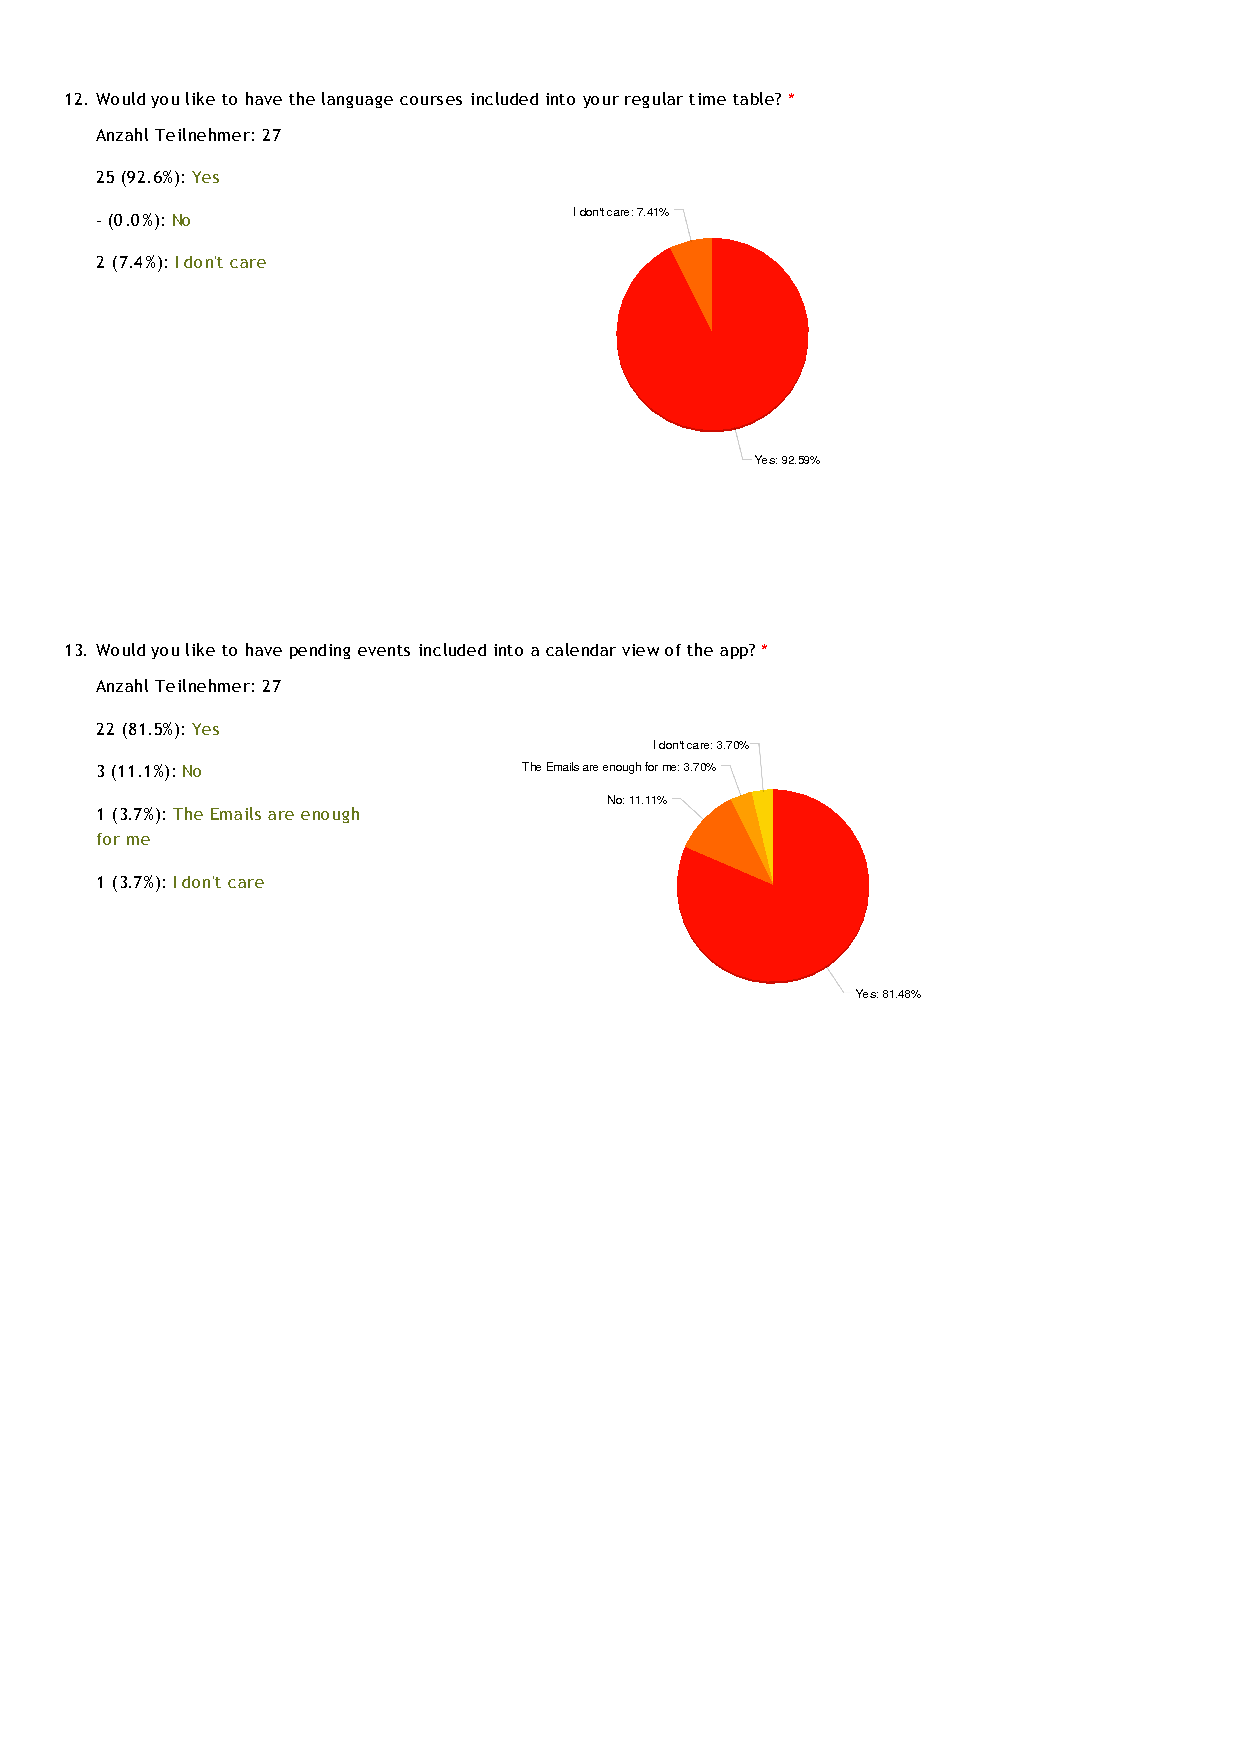
\includegraphics[
    width=\textwidth,
    height=\textheight,
    keepaspectratio
]{Kapiteln/Anhang/Inhalt/EN/survey_EN_Page6.pdf}
\vfill
\newpage
\noindent
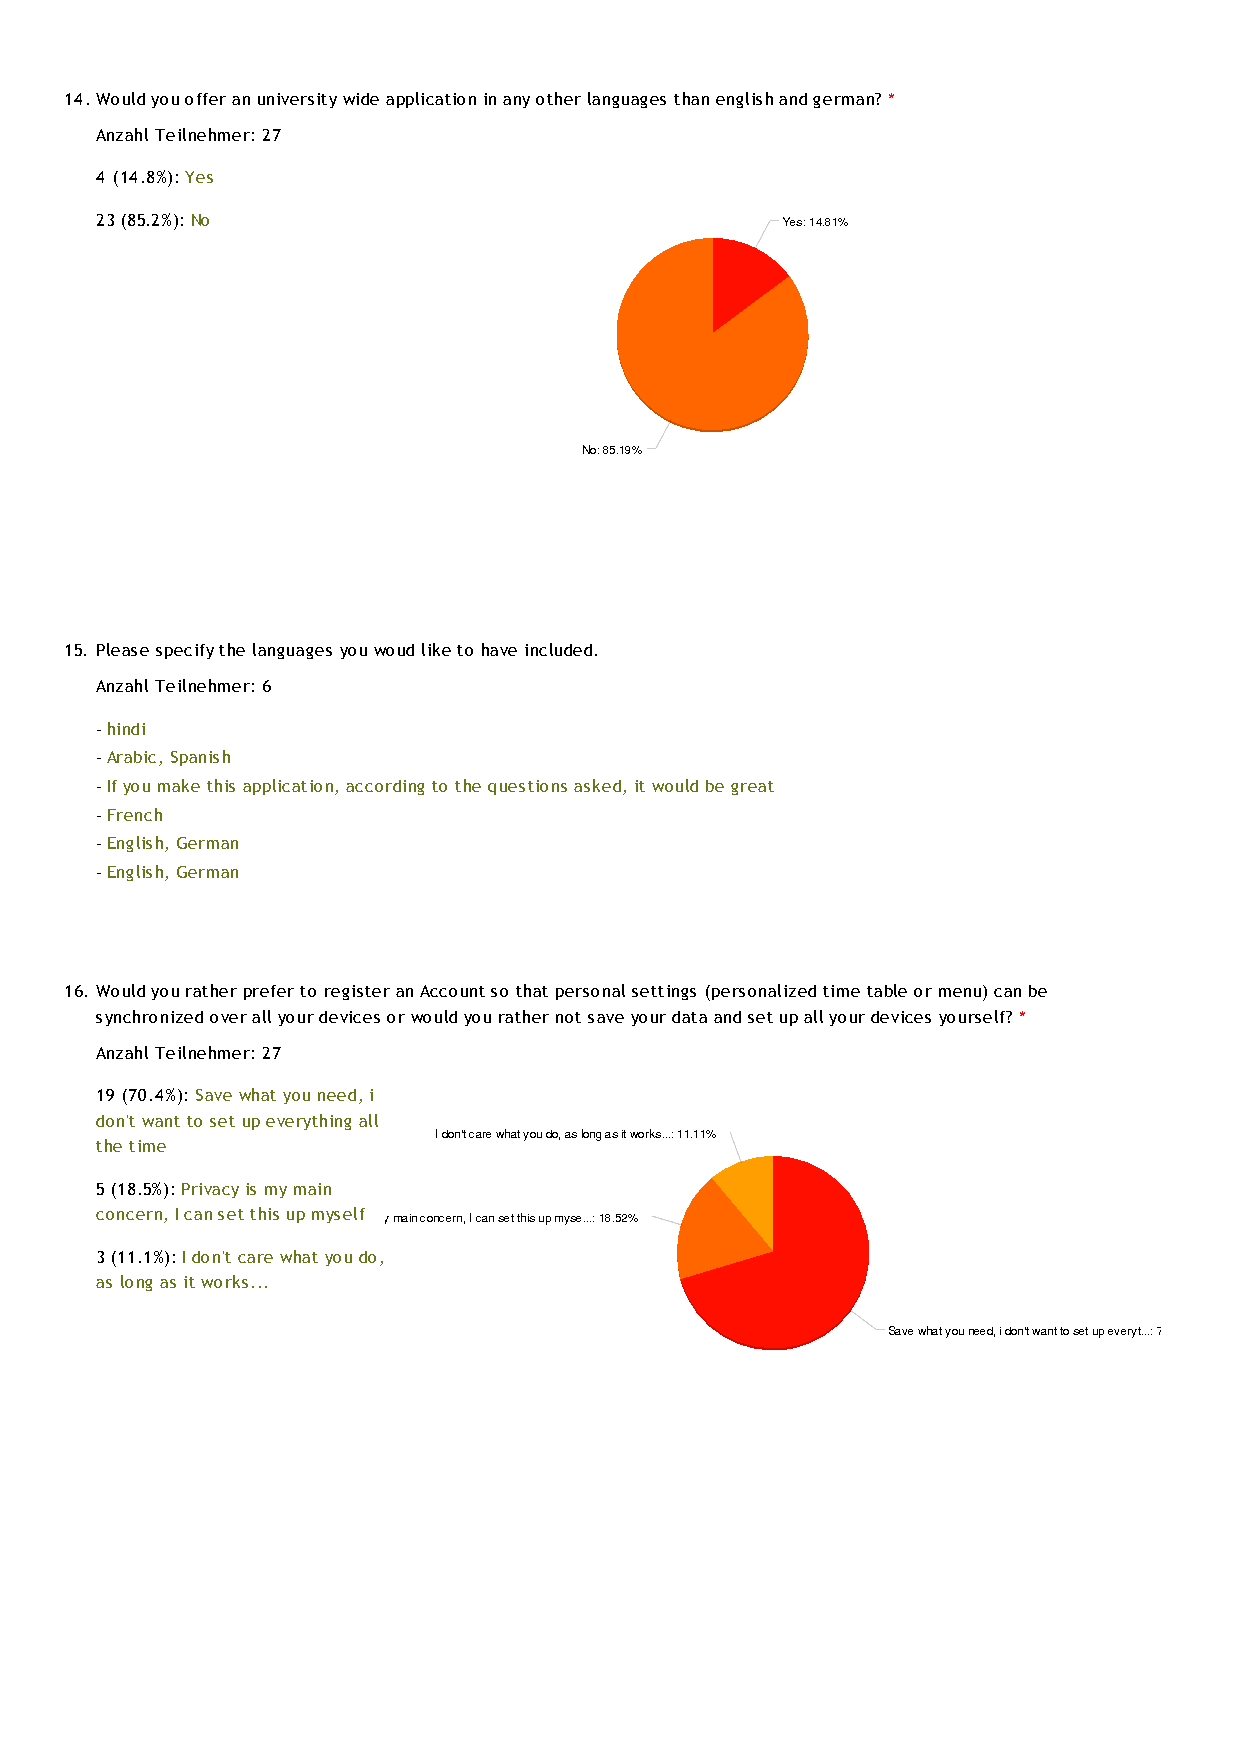
\includegraphics[
    width=\textwidth,
    height=\textheight,
    keepaspectratio
]{Kapiteln/Anhang/Inhalt/EN/survey_EN_Page7.pdf}
\vfill
\newpage
\noindent
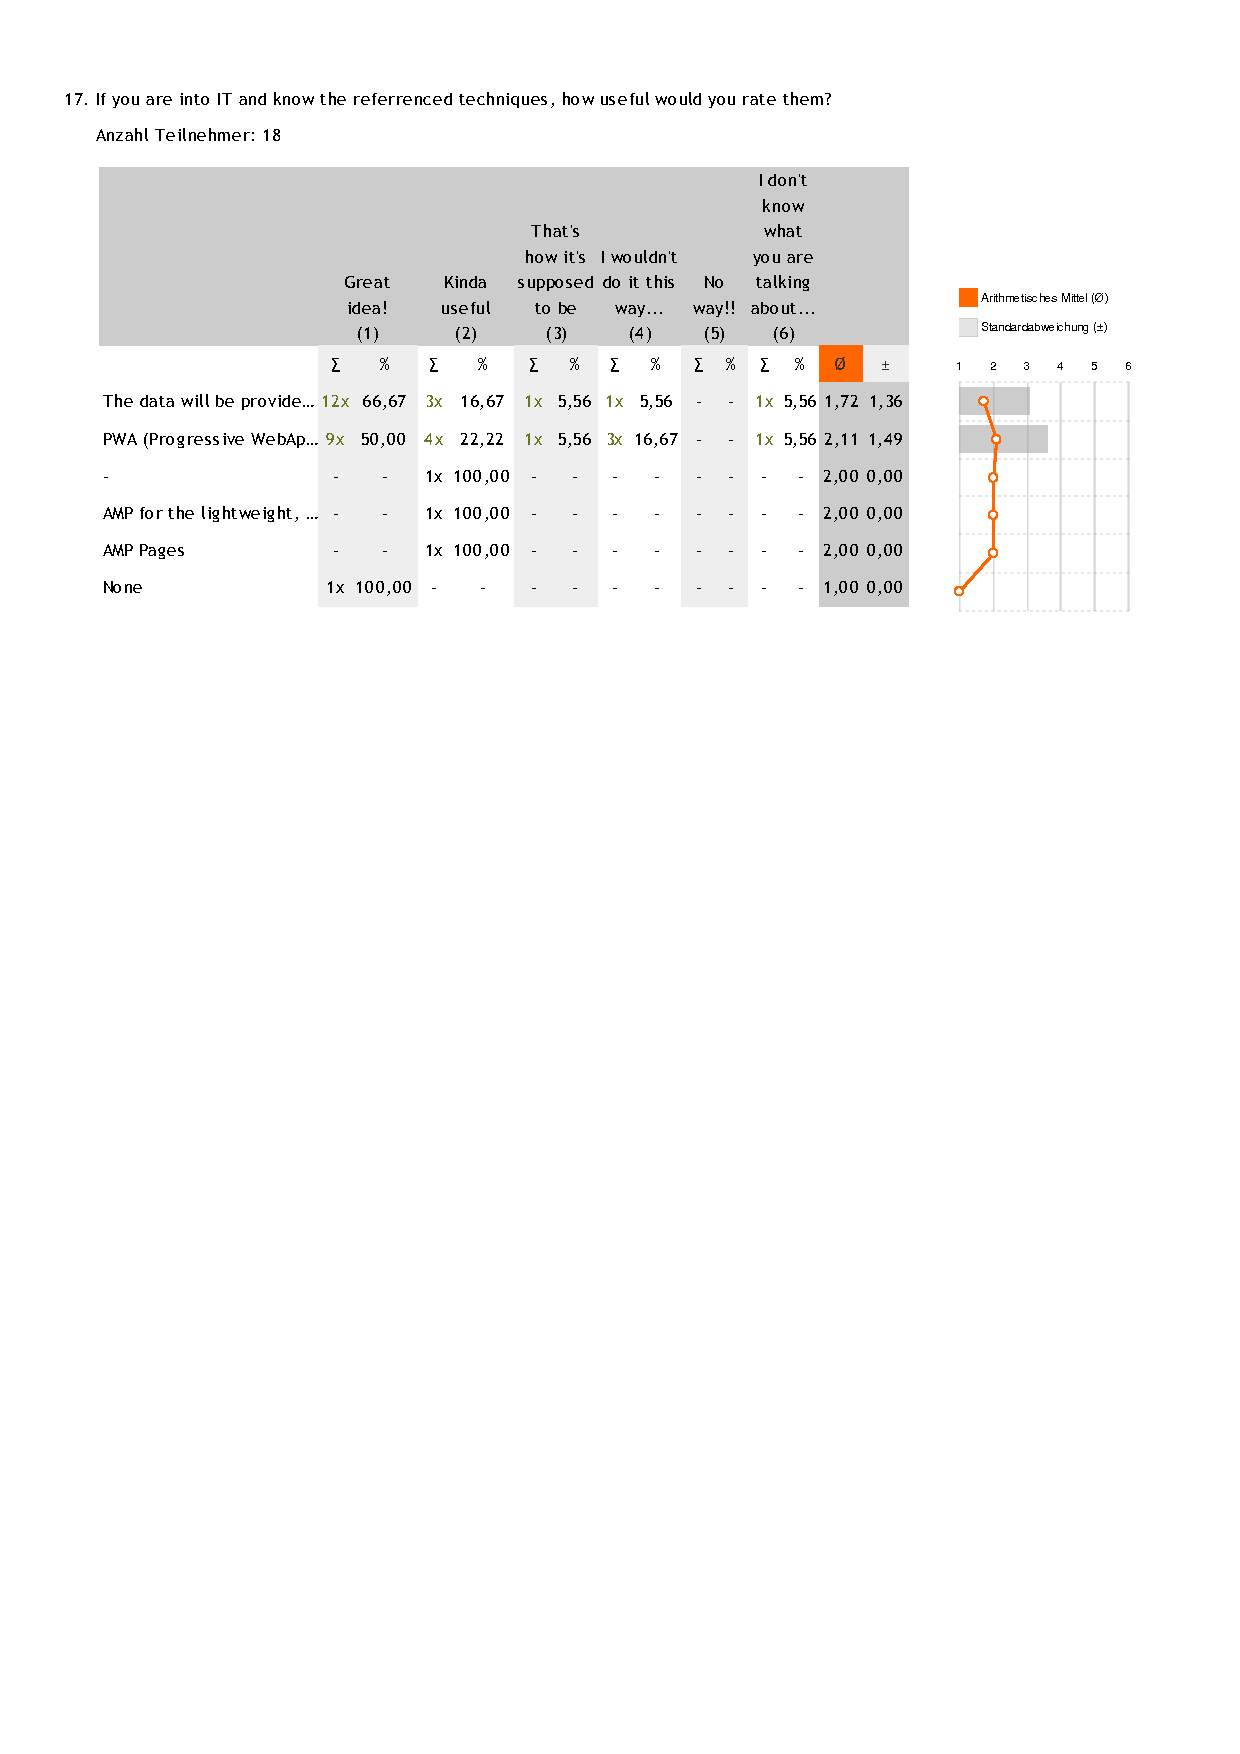
\includegraphics[
    width=\textwidth,
    height=\textheight,
    keepaspectratio
]{Kapiteln/Anhang/Inhalt/EN/survey_EN_Page8.pdf}
\vfill
\cleardoublepage

\section*{Autoren Referenz}
\addcontentsline{toc}{section}{Autoren Referenz}

Diese wissenschaftliche Arbeit ist eine Zusammenarbeit der beiden Autoren Dennis Brysiuk und Noah Lehmann. Um daher einen besseren Überblick über die Zuordnung der Inhalte zu haben wird im folgenden eine Tabelle dargestellt, die die Kapitel ihren jeweiligen Verfassern zuordnet.

\begin{table}[H]
\begin{center}
  \begin{tabular}{| l | l | l |}
 
\hline
\rowcolor{Gray}
\textcolor{white}{\textbf{Kapitel}} & \textcolor{white}{\textbf{Kapitel Bezeichnung}} & \textcolor{white}{\textbf{Autor}} \\
\rowcolor{Gray}
\textcolor{white}{\textbf{Nr.}} 	&  												  & \\  

\hline    
\rowcolor{LGray} 						
\textbf{1}		& \textbf{Einleitung}	&  				\\
\hline
1.1		& Beweggründe					& Noah Lehmann	\\
\hline
1.2		& Zielsetzung					& Noah Lehmann	\\
\hline
1.3		& Zielgruppe					& Noah Lehmann	\\
\hline
1.4		& Vorausgesetztes Wissen		& Noah Lehmann	\\
\hline
1.5		& Vorgeschlagene Nebenlektüre	& Noah Lehmann	\\

\hline    
\rowcolor{LGray} 						
\textbf{2}		& \textbf{Auswertung vorhandener Anwendungen} &  				\\
\hline
2.1		& Allgemeine Auswertung der Zufriedenheit	& Noah Lehmann	\\
\hline
2.1.1	& Zielgruppen								& Noah Lehmann	\\
\hline
2.1.2	& Ergebnisse								& Noah Lehmann	\\
\hline
2.1.3	& Fazit										& Noah Lehmann	\\
\hline
2.2		& Anwendungen								& Noah Lehmann	\\
\hline
2.2.1	& Android									& Noah Lehmann	\\
\hline
2.2.2	& iOS										& Noah Lehmann	\\
\hline
2.2.3	& Windows App								& Noah Lehmann	\\
\hline
2.2.4	& Website									& Noah Lehmann	\\
\hline
2.2.5	& Fazit										& Noah Lehmann	\\

\hline    
\rowcolor{LGray} 						
\textbf{3}	& \textbf{Funktionale Anforderungen} &  				\\
\hline
3.1		& Auftraggeber					& Noah Lehmann	\\
\hline
3.1.1	& Grundlegenden Anforderungen	& Noah Lehmann	\\
\hline
3.1.2	& Funktionale Anforderungen		& Noah Lehmann	\\
\hline
3.2		& International Office			& Noah Lehmann	\\
\hline
3.2.1	& Problem						& Noah Lehmann	\\
\hline
3.2.2	& Funktionale Anforderungen		& Noah Lehmann	\\


\hline
  \end{tabular}
  \end{center}
\caption[Autoren Referenz]{Autoren Referenz}
\label{tab:autoren}
\end{table}

\newpage

\begin{table}[H]
\begin{center}
  \begin{tabular}{| l | l | l |}
 
\hline
\rowcolor{Gray}
\textcolor{white}{\textbf{Kapitel}} & \textcolor{white}{\textbf{Kapitel Bezeichnung}} & \textcolor{white}{\textbf{Autor}} \\
\rowcolor{Gray}
\textcolor{white}{\textbf{Nr.}} 	&  												  & \\  

\hline
3.3		& Sprachenzentrum				& Noah Lehmann	\\
\hline
3.3.1	& Problem						& Noah Lehmann	\\
\hline
3.3.2	& Funktionale Anforderungen		& Noah Lehmann	\\
\hline
3.4		& Pflichtenheft					& Noah Lehmann	\\

\hline    
\rowcolor{LGray} 						
\textbf{4}	& \textbf{Architektur von Softwaresystemen}	&	\\
\hline
4.1		& Grundlegendes						& Dennis Brysiuk \\
\hline
4.2		& Nicht-funktionale Anforderungen	& Dennis Brysiuk \\
\hline
4.3		& Prinzipien						& Dennis Brysiuk \\
\hline
4.3		& Fazit								& Dennis Brysiuk \\

\hline    
\rowcolor{LGray}
\textbf{5}		& \textbf{Web Services}	&  			\\
\hline
5.1		& Serviceorientierte Architektur			& Dennis Brysiuk \\
\hline
5.1.1	& Technische Konzepte						& Dennis Brysiuk \\
\hline
5.1.2	& Zusammenfassung							& Dennis Brysiuk \\
\hline
5.2		& Webservice Arten							& Dennis Brysiuk \\
\hline
5.2.1	& Simple Object Access Protocol (SOAP)		& Dennis Brysiuk \\
\hline
5.2.2	& Representational State Transfer (REST)	& Dennis Brysiuk \\
\hline
5.2.3	& Bewertung									& Dennis Brysiuk \\

\hline    
\rowcolor{LGray}
\textbf{6}		& \textbf{REST API Design}	&  				\\
\hline
6.1		& Ressourcen Design				& Dennis Brysiuk \\
\hline
6.1.1	& Versionsverwaltung			& Dennis Brysiuk \\
\hline
6.1.2	& URI Namenskonvention			& Dennis Brysiuk \\
\hline
6.1.3	& Ressourcen Namenskonvention	& Dennis Brysiuk \\
\hline
6.1.4	& HTTP Methoden					& Dennis Brysiuk \\
\hline
6.2		& Request Struktur				& Dennis Brysiuk \\
\hline
6.2.1	& Header						& Dennis Brysiuk \\
\hline
6.2.2	& Query Parameter				& Dennis Brysiuk \\
\hline
6.2.3	& Aufteilung einer Ressource	& Dennis Brysiuk \\
\hline
6.3		& Response Handling				& Dennis Brysiuk \\
\hline
6.3.1	& Response Inhaltsformat		& Dennis Brysiuk \\
\hline
6.3.2	& HTTP Statuscode				& Dennis Brysiuk \\
\hline
6.3.3	& Asynchrone Callbacks			& Dennis Brysiuk \\
\hline
6.4		& Hypermedia					& Dennis Brysiuk \\

\hline
  \end{tabular}
  \end{center}
\caption[Autoren Referenz]{Autoren Referenz}
\label{tab:autoren}
\end{table}

\newpage

\begin{table}[H]
\begin{center}
  \begin{tabular}{| l | l | l |}
 
\hline
\rowcolor{Gray}
\textcolor{white}{\textbf{Kapitel}} & \textcolor{white}{\textbf{Kapitel Bezeichnung}} & \textcolor{white}{\textbf{Autor}} \\
\rowcolor{Gray}
\textcolor{white}{\textbf{Nr.}} 	&  												  & \\  

\hline    
\rowcolor{LGray} 						
\textbf{7} & \textbf{Architektur Hochschul-App} &  				\\
\hline
7.1		& Serviceorientierte Architektur	& Dennis Brysiuk \\
\hline
7.2		& Microservice Architektur			& Noah Lehmann \\
\hline
7.3		& Schichtenarchitektur				& Noah Lehmann \\

\hline    
\rowcolor{LGray} 						
\textbf{8} & \textbf{Services der Hochschul-App}	&  				\\
\hline
8.1		& Stundenplan (Timetable-Service)			& Noah Lehmann \\
\hline
8.2		& Planänderungen (Timetable-Change-Service)	& Noah Lehmann \\
\hline
8.3		& Speiseplan (Mensa-Service)				& Dennis Brysiuk \\
\hline
8.4		& Benachrichtigungen (Notification Service)	& Dennis Brysiuk \\
\hline
8.5		& Sicherheit (Auth-Service)					& Dennis Brysiuk \\
\hline
8.6		& Anwenderverwaltung (User-Service)			& Dennis Brysiuk \\
\hline
8.7		& Weitere Dienste							& Noah Lehmann \\

\hline    
\rowcolor{LGray} 						
\textbf{9} & \textbf{Ausblick und Fazit} &  				\\
\hline
9.1		& Ausblick						& Noah Lehmann \\
\hline
9.2		& Weitere Bachelorarbeitsthemen	& Noah Lehmann \\
\hline
9.3		& Fazit							& Noah Lehmann \\
\hline

\hline
  \end{tabular}
  \end{center}
\caption[Autoren Referenz]{Autoren Referenz}
\label{tab:autoren}
\end{table}

\cleardoublepage